%%%%%%%%%%%%%%%%%%%%%%%%%%%%%%%%%%%%%%%%%%%%%%%%%%%%%%%%%%%%%%%%%%%%%%%%%%%%%%%%
% \documentclass[12pt,papel,twoside]{ibtesis}
\documentclass[12pt,screen,twoside,pagebackref]{ibtesis}
% \documentclass[12pt,papel,singlespace,oneside]{ibtesis}
% \documentclass[12pt,papel,preprint,singlespace,oneside]{ibtesis}


%%%%%%%%%%%%%%%%%%%%% Paquetes extra %%%%%%%%%%%%%%%%%%%%%%%%%%%%%%%%%%%%%%%%%%%
% Por conveniencia: aqu\'{\i} puede cargar todos los paquetes y definir los comandos 
% que necesite
\usepackage{ibextra}
%%%%%%%%%%%%%%%%%%%%%%%%%%%%%%%%%%%%%%%%%%%%%%%%%%%%%%%%%%%%%%%%%%%%%%%%%%%%%%%%
%%%%%%%%%%%%%%%%%%%%% Informacion sobre la tesis %%%%%%%%%%%%%%%%%%%%%%%%%%%%%%%
\title{Implementación en dispositivos SDR de las etapas de detección y sincronismo
para sistemas inalámbricos que emplean OFDM}
\author{Matías Daniel Roqueta}
\director{Dr.~Juan Pablo Pascual}
\codirector{Ing.~Nicolás Catalano}
\carrera{Tesis Carrera de Ingeniería en Telecomunicaciones}
\grado{Estudiante}
\laboratorio{Departamento de Ingeniería en Telecomunicaciones}
\jurado{Ing. Omelio Barba Leal (Skyloom) \\ 
Ing. José Ignacio Quinteros del Castillo (Emtech)\\
}
\palabrasclave{OFDM, DETECCIÓN, SINCRONISMO, SDR.}
\keywords{OFDM, DETECTION, SYNCHRONIZATION, SDR}
% Si queremos poner la fecha manualmente:
% \date{Diciembre de 2099}

%%%%%%%%%%%%%%%%%%%%%%%%%%%%%%%%%%%%%%%%%%%%%%%%%%%%%%%%%%%%%%%%%%%%%%%%%%%%%%%%
%\titlepagefalse % Si no quiere compilar la portada descomente esta linea
%\includeonly{apendices} % Compilar s\'{o}lo estos archivos 
\graphicspath{{figs/}} % Lugar donde encontrar las figuras generales (se puede poner uno en cada cap{\'{\i}}tulo)
%%%%%%%%%%%%%%%%%%%%%%%%%%%%%%%%%%%%%%%%%%%%%%%%%%%%%%%%%%%%%%%%%%%%%%%%%%%%%%%%


\begin{document}

% Dentro del environment 'preliminary' va:
% la dedicatoria, resumen, abstract, indices

\begin{preliminary}

% Escriba su dedicatoria
\dedicatoria{
A mi familia\\
A mis amigos\\
A todos los que me conocen\\
A toda esa otra gente que no
}

%%% \'{I}ndices %%%%

\begin{abreviaturas}
  \begin{description}[labelwidth=2cm,leftmargin=!]
    \item[BPSK:]  \textit{Binary Phase Shift Key} - Desplazamiento de fase binario
    \item[CPU:]   \textit{Central Processing Unit} - Unidad central de procesamiento
    \item[FFT:]   \textit{Fast Fourier Transform} - Transformada rápida de Fourier
    \item[FIFO:]  \textit{First In, First Out} - Primero en entrar, primero en salir
    \item[FPGA:]  \textit{Field Programmable Gate Array} - Matriz de compuertas lógicas programable
    \item[FLOPS:] \textit{Floating Point Operations per Second} - Operaciones de punto flotante por segundo
    \item[GI:]    \textit{Guard Interval} - Intervalo de guarda
    \item[IEEE:]  \textit{Institute of Electrical and Electronic Engineering}
    \item[ISI:]   \textit{Inter-Symbol Interference} - Interferencia entre símbolos
    \item[ITU:]   \textit{International Telecommunications Union} - Unión Internacional de las Telecomunicaciones
    \item[IFFT:]  \textit{Inverse Fast Fourier Transform} - Antitransformada rápida de Fourier
    \item[MSE:]   \textit{Mean Square Error} - Error cuadrático medio
    \item[MVUE:]  \textit{Minimum Variance Unbiased Estimator} - Estimador insesgado de mínima varianza
    \item[NI:]    \textit{National Instruments}
    \item[OFDM:]  \textit{Orthogonal Frequency Division Multiplexing} - Multiplexación por división en frecuencias ortogonales
    \item[PHY:]   \textit{Physical Layer} - Capa física
    \item[PPDU:]  \textit{PHY Protocol Data Unit} - Unidad de datos del protocolo de capa física
    \item[QAM:]   \textit{Quadrature Amplitude Modulation} - Modulación de amplitudes en cuadratura
    \item[RF:]       \textit{Radio Frecuency} - Radiofrecuencia
    \item[QPSK:]  \textit{Quadrature Phase Shift Key} - Desplazamiento de fase en cuadratura 
    \item[SDR:]   \textit{Software Defined Radio} - Radio definida por software
    \item[SNR:]   \textit{Signal to Noise Ratio} - Relación de señal a ruido
    \item[USRP:]  \textit{Universal Software Radio Peripheral} - Periférico universal de radio programable
  \end{description}
\end{abreviaturas}

\tableofcontents                %\'{I}ndice

\listoffigures                  %Figuras

\listoftables                   %Tablas

\begin{resumen}%

La recepción de señales inalámbricas en todo sistema de comunicaciones inicia con las etapas de detección y sincronismo, las cuales necesitan ejecutarse en línea durante la operación del sistema. En la transmisión empleando OFDM de acuerdo al estándar IEEE 802.11 se especifican las características que debe tener de una trama transmitida para permitir que el receptor implemente estas etapas. En el presente trabajo se describe el desarrollo e implementación de algoritmos de detección y sincronismo diseñados para operar en línea sobre un dispositivo SDR utilizando LabVIEW. 

En la primera etapa del trabajo se estudian las especificaciones para la transmisión con OFDM definidas por el estándar IEEE 802.11a, las cuales habilitan la detección y sincronismo por medio de la inclusión del preámbulo de capa física a las trama transmitidas. Además, se toma consideración de las especificaciones del estándar referentes a las escalas de tiempo y frecuencia usadas en la transmisión.

La segunda y la tercera etapa se centran en estudiar los algoritmos de sincronismo y detección respectivamente, los cuales que se desarrollan en base al conocimiento del preámbulo de capa física. Se verifica el correcto funcionamiento de los algoritmos y se procede a implementarlos en LabVIEW.

La etapa final consiste en la implementación de un sistema que integra los algoritmos implementados durante la etapa anterior, analizando posibles fuentes de error propias a la operación en línea y aplicando estrategias para evitar a las mismas. Se verifica una prueba de concepto del sistema diseñado, se prueba si éste es capaz de alcanzar la tasa de iteraciones mínima requerida para la operación en tiempo real, y se analizan los pasos futuros requeridos para lograr que éste diseño sea capaz de alcanzar la tasa de iteraciones necesaria.

\end{resumen}

\begin{abstract}%
This is the title in English:\\
The thesis must reflect the work of the student, including the chosen methodology, the results and the conclusions that those results allow us to draw.
\end{abstract}


%%% Local Variables: 
%%% mode: latex
%%% TeX-master: "template"
%%% End: 


\end{preliminary}


% Podemos usar cualquiera de los dos comandos: \input o \include para incluir el texto
\chapter{Introducción}
\label{Ch:1}
\graphicspath{{figs/}}
\chapterquote{Hablaban siempre de dinero y planeaban asaltar un banco}{Domingo Cavallo, 2001}

\section{Antecedentes}
\label{S:ch1-antecedentes}

\section{Objetivos}
\label{S:ch1-objetivos}

\section{Organización de la Tésis}
\label{S:ch1-organización}

%%% Local Variables: 
%%% mode: latex
%%% TeX-master: "template"
%%% End: 

\chapter{Transmisión OFDM en Estándar IEEE 802.11a}
\label{Ch:2}
\graphicspath{{figs/}}

En la sección 17.3 del estándar IEEE 802.11\cite{ieee} se definen las especificaciones a nivel físico de la transmisión empleando señales que utilizan OFDM. El estándar define las técnicas utilizadas para traducir los datos provenientes de capas superiores a formas de ondas que se transmitirán por el medio inalámbrico utilizando OFDM, así como los métodos utilizados para asegurar que el receptor sea capaz de reconocer e interpretar las señales transmitidas.

En este capítulo se resumen los aspectos del estándar IEEE 802.11 relevantes para el desarrollo del proyecto, partiendo de la descripción de la unidad fundamental de la señal, el símbolo OFDM.

Una vez definido el símbolo OFDM, se procede a describir la estructura de la trama que se transmitirá por el medio inalámbrico, que recibe el nombre de unidad de datos del protocolo de capa física (PPDU por sus siglas en inglés).

Finalmente, se detalla el formato la primera parte de la PPDU, llamada preámbulo. Esta cumple la función de facilitar la detección y el sincronismo de la señal en el receptor, por lo que es de especial importancia para este proyecto.

\section{Símbolo OFDM}
\label{S:ch2-simbolo}

El símbolo OFDM es la unidad fundamental de la señal transmitida en cada trama. La construcción del mismo se basa en especificaciones tanto en el dominio de la frecuencia como en el dominio del tiempo.

Las componentes en frecuencia se transforman al dominio del tiempo en una ventana temporal de duración definida por el estándar. 

\subsection{Subportadoras}
\label{Ss:ch2-subportadoras}

Un símbolo OFDM se construye a partir de 52 componentes en frecuencia, que reciben el nombre subportadoras, de las cuales 48 transportan datos y las 4 restantes transportan tonos pilotos. 

Los datos transportados en el símbolo llevan índice de 0 a 47, y son números complejos que representan las coordenadas de los bits de un mensaje en una constelación de modulación, la cual puede ser BPSK, QPSK, 16-QAM, o 64-QAM. Los tonos pilotos toman los valores de una secuencia pseudoaleatoria predefinida modulada en BPSK, estos tienen el propósito de preservar el sincronismo durante la recepción con métodos que exceden el alcance de este proyecto.

Las 52 subportadoras, a su vez, son indexadas simétricamente, de -26 a 26, omitiendo el 0 que siempre lleva valor nulo. Las subportadoras de índice -21, -7, 7, y 21 son reservadas para los tonos pilotos y las restantes son asignadas los datos según el mapa descrito en la Figura \ref{fig:asignacion-subportadoras}
\begin{figure}[t]
    \centering{}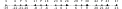
\includegraphics[width=\imsizeL]{asignacion_subportadoras.pdf}
    \caption{Mapa de asignación de datos según sus índices a las subportadoras que constituyen un símbolo OFDM.\label{fig:asignacion-subportadoras}}  
\end{figure}

\subsection{Duración temporal del símbolo}
\label{Ss:ch2-tiempo-simbolo}

\begin{table}[t]
    \centering{}
    \begin{tabular}{|l|l|l|}
    \hline
     \thead{Parámetro} & \thead{Significado} & \thead{Fórmula}\\
     \hline
     $T_{FFT}$ & Duración de los intervalos de IFFT y FFT. & $1/\Delta_F$  \\
     $T_{GI}$  & Intervalo de guarda para los símbolos OFDM. & $T_{FFT}/4$      \\
     $T_{SYM}$ & Duración de un símbolo OFDM. & $T_{GI}+T_{FFT}$ \\
     $T_{GI2}$ & Intervalo de guarda para los campos del preámbulo. & $T_{FFT}/2$      \\
     $T_{SHORT}$ & Duración de la primera secuencia de entrenamiento. & $10\times T_{FFT}/4$  \\
     $T_{LONG}$  & Duración de la segunda secuencia de entrenamiento. & $T_{GI2}+2\times T_{FFT}$ \\
     \hline
    \end{tabular}
    \caption{Parámetros temporales relevantes a la transmisión con OFDM en el estándar IEEE 802.11a y sus fórmulas en función del parámetro $\Delta_F$.\label{tab:tiempos-formula}}
\end{table}

\begin{table}[t]
    \centering{}
    \begin{tabular}{|l|c|c|c|}
    \hline
     \thead{Parámetro} & \thead{Valor con canales\\espaciados 20 MHz}& \thead{Valor con canales\\espaciados 10 MHz} & \thead{Valor con canales\\espaciados 5 MHz} \\
     \hline
     $T_{FFT}$   & $3.2$ \textmu s & $6.4$ \textmu s & $12.8$ \textmu s \\
     $T_{GI}$    & $0.8$ \textmu s & $1.6$ \textmu s & $3.2$ \textmu s \\
     $T_{GI2}$   & $1.6$ \textmu s & $3.2$ \textmu s & $6.4$ \textmu s \\
     $T_{SYM}$   & $4$ \textmu s & $8$ \textmu s & $16$ \textmu s \\
     $T_{SHORT}$ & $8$ \textmu s & $16$ \textmu s & $32$ \textmu s \\
     $T_{LONG}$  & $8$ \textmu s & $16$ \textmu s & $32$ \textmu s \\
     \hline
    \end{tabular}
    \caption{Valores de los parámetros temporales según los valores de espaciamiento entre canales admitidos por el estándar IEEE 802.11a.\label{tab:tiempos-valor}}
\end{table}


En función del espacio entre subportadoras, $\Delta_F$, el estándar define distintos intervalos temporales que resultan de interés. Dichos parámetros se resumen en la Tabla \ref{tab:tiempos-formula}. El parámetro $\Delta_F$ es determinado por el espaciamiento entre canales en el dominio de la frecuencia, específicamente es el resultado de dividir entre 64 la separación entre los canales.

En el funcionamiento típico, los canales están espaciados 20 MHz, pero también se admite operación con espaciamiento de 10 MHz y con espaciamiento de 5 MHz. La longitud de los intervalos temporales son inversamente proporcionales al espaciamiento entre canales, y sus valores se detallan en la Tabla \ref{tab:tiempos-valor}.



\subsection{IFFT}
\label{Ss:ch2-ifft}

\begin{figure}[t]
    \centering
    \hfill
    \subcaptionbox{Aplicación de IFFT de 64 puntos.\label{fig:ifft64}}{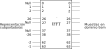
\includegraphics[width=0.5\imsizeL]{IFFT.pdf}}%
    \hfill
    \subcaptionbox{Aplicación de IFFT de 128 puntos.\label{fig:ifft128}}{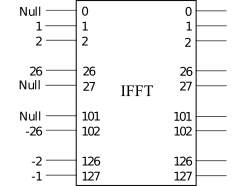
\includegraphics[width=0.5\imsizeL]{IFFT128.pdf}}%
    \caption{Esquema de aplicación de IFFT a una descripción en subportadoras de un símbolo OFDM.\label{fig:ifft}}
    \hfill
\end{figure}

La representación en subportadoras de un símbolo OFDM se transforma al dominio del tiempo con un módulo IFFT. Típicamente, se utilizan módulos IFFT con un número de puntos potencia de 2 necesariamente mayor o igual a 64, el número de puntos utilizados recibe el nombre $N_{FFT}$. Para obtener una correcta transformación del dominio se aplica una operación de desplazamiento, transportando las subportadoras de índice negativo al final del vector de entrada del módulo IFFT. Este desplazamiento se esquematiza en la Figura \ref{fig:ifft}.

En el estándar se define la transformación con $N_{FFT}=64$, sin embargo, \color{Green} es posible aplicar el mismo desplazamiento considerando un valor de $N_{FFT}$ mayor \color{black} y resulta en una mayor resolución temporal de la señal. Cabe destacar que independientemente del valor de $N_{FFT}$, la duración temporal de la salida es el valor $T_{FFT}$ definido en la Tabla \ref{tab:tiempos-valor}, y el espacio entre las muestras valdrá $T_S = T_{FFT}/N_{FFT}$.

\subsection{Prefijo cíclico}
\label{Ss:ch2-prefijo}
\begin{figure}[t]
    \centering{}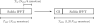
\includegraphics[width=\imsizeL]{prefix.pdf}
    \caption{Diagrama de aplicación de intervalo de guarda a un símbolo OFDM.\label{fig:prefijo}}  
\end{figure}


Al vector resultante de la operación IFFT se le agrega un intervalo de guarda, (GI por sus siglas en inglés), el cual tiene la función de mitigar efectos de interferencia entre símbolos (ISI por sus siglas en inglés). El GI consiste en un prefijo cíclico de la señal temporal, y se construye de la siguiente forma: se toman las últimas $N_{FFT}/4$ muestras de la señal, y se las concatena al inicio de las $N_{FFT}$ muestras existentes. Este procedimiento se representa gráficamente en la Figura \ref{fig:prefijo}. La inclusión del prefijo cíclico completa la estructura del símbolo OFDM que será transmitido.


\section{Estructura de la PPDU}
\label{S:ch2-ppdu}

\begin{figure}[t]
    \centering{}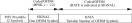
\includegraphics[width=\imsizeL]{PPDU.pdf}
    \caption{Estructura de alto nivel de una PPDU en el estándar IEEE 802.11.\label{fig:ppdu}}  
\end{figure}

La PPDU consiste en una secuencia de símbolos OFDM que transmiten un mensaje a través de la capa física, la cual se describe en la Figura \ref*{fig:ppdu}, esta incorpora a un mensaje la información requerida para detección, sincronismo, demodulación, y decodificación del mismo. Los campos que la constituyen son los siguientes:

\begin{enumerate}
    \item PHY Preamble: secuencia de símbolos OFDM predeterminados utilizados para detección, sincronismo, y estimación del canal.
    \item SIGNAL: símbolo OFDM que transmite la información necesaria para la recepción de DATA a través de los campos LENGTH y RATE. Siempre es modulado en BPSK y codificado a tasa 1/2.
    \item DATA: número variable de símbolos OFDM que transmiten la información del mensaje propiamente dicha, el número de símbolos es informado por LENGTH, y la modulación de cada subportadora y tasa del código de correción de errores utilizados son determinadas únivocamente por RATE.
\end{enumerate}

El campo PHY Preamble cumple un rol fundamental en lo que hace a la detección y sincronismo tanto en tiempo como en frecuencia en el receptor,  por lo que se hará énfasis en su estructura a lo largo de este trabajo. En cambio, las funciones y estructuras de los campos SIGNAL y DATA exceden el alcance del proyecto, por lo que no se estudiarán en mayor detalle.

\section{PHY Preamble}
\label{S:ch2-preambulo}

El preámbulo es una forma de onda predeterminada transmitida al inicio de cada PPDU. Este consiste en dos secuencias, las cuales se construyen de forma similar a otros símbolos, pero en lugar de contener datos y tonos pilotos, las 52 subportadoras \color{Red} tienen asignados \color{black} valores predefinidos. Las dos secuencias reciben el nombre de secuencia de entrenamiento de símbolos cortos y secuencia de entrenamiento de símbolos largos, y las asignaciones de subportadoras usadas para construirlas son definidas por los vectores $S$ y $L$ respectivamente:
\begin{align}
    &\begin{aligned}
        S_{-26,26} = \sqrt{13/6}\times 
        [&0 ,\,  0   ,\, 1+j ,\,  0   ,\, 0 ,\,  0   ,\, -1-j ,\,  0   ,\, 0 ,\, 0   ,\, 1+j ,\, 0   ,\, 0 ,\, 
         0 ,\, -1-j ,\, 0   ,\,  0   ,\, 0 ,\\ 
         &-1-j ,\,  0   ,\,  0   ,\, 0 ,\, 1+j ,\, 0   ,\, 0   ,\, 0 ,\, 0 ,\,
         0 ,\,  0   ,\, 0   ,\, -1-j ,\, 0 ,\,  0   ,\,  0   ,\, -1-j ,\\ 
         &0 ,\, 0   ,\, 0   ,\, 1+j ,\, 0 ,\, 
         0 ,\,  0   ,\, 1+j ,\,  0   ,\, 0 ,\,  0   ,\,  1+j ,\,  0   ,\, 0 ,\, 0   ,\, 1+j ,\, 0   ,\, 0],
    \end{aligned}\label{eq:def-S}\\
    &
    \begin{aligned}
        L_{-26,26} = 
        [&1,\, 1,\, -1,\, -1,\, 1,\, 1,\, -1,\, 1,\, -1,\, 1,\, 1,\, 1,\, 1,\, 1,\, 1,\, -1,\, -1, 1,\, 1,\, -1,\, 1,\, -1,\, 1,\\& 1,\, 1,\, 1,\, 
        0,\,
        1,\, -1,\, -1,\, 1,\, 1,\, -1,\, 1,\, -1,\, 1, -1,\, -1,\, -1,\, -1,\, -1,\, 1,\, 1,\, -1,\\& -1,\, 1,\, -1,\, 1,\, -1,\, 1,\, 1,\, 1,\, 1].
    \end{aligned}\label{eq:def-L}
\end{align}
\begin{figure}[t]
    \centering{}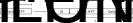
\includegraphics[width=\imsizeL]{training_symbol.pdf}
    \caption{Diagrama de aplicación de intervalo de guarda a una secuencia de entrenamiento del preámbulo.\label{fig:training-symbol}}  
\end{figure}

A diferencia de los símbolos OFDM pertenecientes a los campos SIGNAL y DATA, las secuencias de entrenamiento tienen el doble de duración, establecida por los valores $T_{SHORT}$ y $T_{LONG}$ registrados en la Tabla \ref{tab:tiempos-valor}. Su intervalo de guarda también tiene el doble de duración, definida por $T_{GI2}$. El procedimiento para construir una secuencia de entrenamiento a partir de la salida del módulo IFFT se describe en la Figura \ref{fig:training-symbol}.

\subsection{Secuencia de entrenamiento de símbolos cortos}
\label{Ss:ch2-short}
%\begin{equation}\label{eq:def-S}
%    \begin{aligned}
%    S_{-26,26} = \sqrt{13/6}\, 
%    [0 ,\,  0   ,\, 1+j ,\,  0   ,\, 0 ,\,  0   ,\, -1-j ,\,  0   ,\, 0 ,\, 0   ,\, 1+j ,\, 0   ,\, 0 ,\, 
%     0 ,\, -1-j ,\, 0   ,\,  0   ,\, 0 ,\\ -1-j ,\,  0   ,\,  0   ,\, 0 ,\, 1+j ,\, 0   ,\, 0   ,\, 0 ,\, 0 ,\,
%     0 ,\,  0   ,\, 0   ,\, -1-j ,\, 0 ,\,  0   ,\,  0   ,\, -1-j ,\\ 0 ,\, 0   ,\, 0   ,\, 1+j ,\, 0 ,\, 
%     0 ,\,  0   ,\, 1+j ,\,  0   ,\, 0 ,\,  0   ,\,  1+j ,\,  0   ,\, 0 ,\, 0   ,\, 1+j ,\, 0   ,\, 0]
%    \end{aligned}
%\end{equation}

\begin{figure}[t]
    \centering{}\includegraphics[width=\imsize]{short_sc.pdf}
    \caption{Asignación de subportadoras para la construcción de la secuencia de entrenamiento de símbolos cortos.\label{fig:short-sc}}  
\end{figure}
\begin{figure}[t]
    \centering{}\includegraphics[width=\imsize]{short_time.pdf}
    \caption[Secuencia de entrenamiento de símbolos cortos en el dominio temporal.]{Secuencia de entrenamiento de símbolos cortos en el dominio temporal, usando $T_{SHORT} = 8$ \textmu s y una IFFT de 64 puntos.\label{fig:short-time}}  
\end{figure}

La secuencia de entrenamiento de símbolos cortos representa la primera mitad del preámbulo, construida a partir del resultado de aplicar la IFFT a la secuencia $S$ definida en la Ecuación \ref{eq:def-S}. Esta secuencia asigna valores complejos únicamente a subportadoras con índices múltiplos de 4, la secuencia se grafica en la Figura \ref{fig:short-sc}.

Aplicar la IFFT a $S$ y agregar el intervalo de guarda produce una señal con un período de duración $T_{FFT}/4$, el cual recibe el nombre de símbolo corto. La secuencia de entrenamiento de símbolos cortos contiene 10 de estos símbolos y es graficada en la Figura \ref{fig:short-time}. Esta secuencia cumple la función de facilitar la detección de la señal entrante en el receptor, así como permitir algoritmos preliminares de sincronismo, y es de vital importancia para este proyecto.

\subsection{Secuencia de entrenamiento de símbolos largos}
\label{Ss:ch2-long}
%\begin{equation}\label{eq:def-L}
%    \begin{aligned}
%    L = 
%    [1,\, 1,\, -1,\, -1,\, 1,\, 1,\, -1,\, 1,\, -1,\, 1,\, 1,\, 1,\, 1,\, 1,\, 1,\, -1,\, -1,\\
%    1,\, 1,\, -1,\, 1,\, -1,\, 1,\, 1,\, 1,\, 1,\, 
%    0,\,
%    1,\, -1,\, -1,\, 1,\, 1,\, -1,\, 1,\, -1,\, 1,
%    \\ -1,\, -1,\, -1,\, -1,\, -1,\, 1,\, 1,\, -1,\, -1,\, 1,\, -1,\, 1,\, -1,\, 1,\, 1,\, 1,\, 1]
%    \end{aligned}
%\end{equation}
    
\begin{figure}[t]
    \centering{}\includegraphics[width=\imsize]{long_sc.pdf}
    \caption{Asignación de subportadoras para la construcción de la secuencia de entrenamiento de símbolos largos.\label{fig:long-sc}}
\end{figure}
\begin{figure}[t]
    \centering{}\includegraphics[width=\imsize]{long_time.pdf}
    \caption[Secuencia de entrenamiento de símbolos largos en el dominio temporal.]{Secuencia de entrenamiento de símbolos largos en el dominio temporal, usando $T_{LONG} = 8$ \textmu s y una IFFT de 64 puntos..\label{fig:long-time}}  
\end{figure}

La secuencia de entrenamiento de símbolos largos representa la segunda mitad del preámbulo. La IFFT es aplicada a la secuencia $L$ definida en la Ecuación \ref{eq:def-L} la cual se grafica en la Figura \ref{fig:long-sc}. A diferencia de $S$, esta asigna valores reales a todas las subportadoras.

En este caso, aplicar la IFFT produce el símbolo largo de duración $T_{FFT}$, y la secuencia de entrenamiento de símbolos largos la cual es graficada en la Figura \ref{fig:long-time} consiste en 2.5 de estos símbolos. Sus funciones incluyen permitir algoritmos de sincronismo fino en el receptor, así como funciones de estimación de la respuesta al impulso del canal.


\section{Resumen del capítulo}

En el capítulo se resumieron las características de las señales que emplean OFDM de acuerdo con el estándar \color{Red} IEEE 802.11a \color{black} que son necesarias para poder llevar adelante el proyecto. Se detalla el procedimiento para construir un símbolo OFDM a partir de una secuencia de coordenadas resultantes de una constelación de modulación y cómo estos símbolos se organizan para formar una PPDU.

Se presta particular atención al campo PHY Preamble, específicamente a su primer mitad, la secuencia de entrenamiento de símbolos cortos. Conocer la forma y las propiedades de esta secuencia de entrenamiento permite implementar algoritmos de detección y sincronismo, \color{Red} tal como se describe \color{black} en los capítulos siguientes.

%%% Local Variables: 
%%% mode: latex
%%% TeX-master: "template"
%%% End: 

\chapter{Métodos de sincronismo}
\label{Ch:3}
\graphicspath{{figs/}}

Este capítulo se centra en el problema de sincronismo. En la primera sección se define el sincronismo en sistemas que emplean OFDM con la especificación de dos tipos de error de sincronismo que afectan el desempeño de los sistemas: el desvío de temporización de símbolo y el desvío de frecuencia de portadora. 

En la segunda sección se describen dos métodos para estimar los errores de sincronismo en cuestión: el banco de correladores y el algoritmo \textit{delay and correlate}. Finalmente, en la tercera sección se detalla cómo se implementaron estos métodos en LabVIEW, incluyendo diagramas en bloques de los algoritmos descritos en la sección anterior.

\section{Sincronismo en sistemas OFDM}
\label{S:ch3-sincronismo}

En todo medio de transmisión resolver el problema de sincronismo es fundamental para permitir la correcta intrerpretación de la señal por parte del receptor. Se dice que el receptor no está sincronizado cuando éste desconoce los parámetros que son necesarios para recuperar una señal en banda base a partir de la recepción de esta señal en radiofrecuencia. Una desviación entre un parámetro supuesto por el receptor y el ideal que permitirá la recepción óptima recibe el nombre de error de sincronismo, y sincronizar el receptor consiste en estimar los valores de éstos parámetros y aplicar correcciones que permitan minimizar los errores.

Existen cuatro tipos de error de sincronismo principales que afectan la recepción de señales OFDM: desvío de temporización de símbolo, desvío de reloj de muestreo, desvío de frecuencia de portadora, y error de fase de portadora \cite{chiueh}. En el proyecto se implementarán algoritmos para sincronizar el desvío de de temporización de símbolo y el desvío de frecuencia de portadora.

\subsection{Desvío de temporización de símbolo}
\label{Ss:ch3-sincronismo-tiempo}

Se ha visto que la transmisión empleando OFDM consiste en el envío consecutivo de símbolos, construídos por una operación IFFT y la aplicación de un intervalo de guarda. Para recuperar los valores asignados a las subportadoras, el receptor debe realizar el proceso inverso a la generación del símbolo, es decir, remover la guarda y aplicar una operación FFT al intervalo correspondiente al resultado de la IFFT realizado por el transmisor.

En la práctica, los canales inalámbricos distorsionan la señal transmitida, llevando a que las muestras correspondientes a un símbolo contaminen las muestras pertenecientes a símbolos siguientes. El intervalo de guarda cumple la función de permitir que la respuesta al impulso del canal se extinga antes de la ventana FFT que aplicará el receptor, con el propósito de las muestras del símbolo previo no influyan en las muestras que se llevarán al dominio transformado. La interferencia entre símbolos (ISI por sus siglas en inglés) existe cuando la ventana FFT aplicada por el receptor se desvía respecto a la ideal, ya sea si esta se adelanta y toma muestras pertenecientes al símbolo siguiente, o si se atrasa y toma muestras afectadas por el símbolo previo. Este efecto se esquematiza en la Figura \ref{fig:ventana-fft}.
\begin{figure}[t]
    \centering{}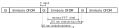
\includegraphics[width=\imsizeL ]{ventana-fft.pdf}
    \caption{Diagrama temporal de aplicación de ventana FFT a una secuencia de símbolos OFDM recibidos, describiendo la ventana ideal y los casos en los que una desviación temporal produce interferencia entre símbolos.\label{fig:ventana-fft}}  
\end{figure}

Sabiendo la duración de un símbolo OFDM y suponiendo que el reloj del receptor está suficientemente sincronizado con el reloj del transmisor, se espera que la ventana FFT esté correctamente sincronizada si se determina precisamente la muestra en la que inicia la trama recibida, por lo que identificar esta muestra es el paso inicial para evitar desvíos en temporización de símbolo.

\subsection{Desvío de frecuencia de portadora}
\label{Ss:ch3-sincronismo-frecuencia}

En los sistemas de comunicaciones digitales la señal digital equivalente en banda base que contiene la información a transmitir, $x[n]$. Al resultado de convertir la señal digital al dominio analógico se le conoce como envolvente compleja, $x(t)$, y suele representarse a través de sus componentes en fase, $x_I(t)$, y en cuadratura, $x_Q(t)$, por medio de la relación
\begin{equation}
    x(t) = x_I(t)+jx_Q(t),
\end{equation}
mientras que la señal elevada a radiofrecuencia que se transmite por el canal inalámbrico recibe el nombre de $x_R(t)$, y tiene las siguientes componentes
\begin{equation}
    x_R(t) = x_I(t)\cos(2\pi f_c t) + x_Q(t)\sin(2\pi f_c t),
\end{equation}
en donde $f_C$ es la frecuencia de portadora.

El receptor demodula $x_R(t)$ con con un demodulador coherente tal como el que se observa en la Figura \ref{fig:demod-err}, el cual utiliza osciladores locales. En una transmisión ideal el oscilador local conoce $f_C$, lo cual permite recuperar exactamente $x[n]$, siendo $x[n]=x(nT_s)$ la digitalización de la envolvente compleja a un intervalo de muestreo $T_s$. Sin embargo, oscilador local del demodulador coherente que utiliza el receptor tiene una frecuencia propia la cual se puede expresar como $f_c+\Delta f$, donde $\Delta f$ denota un error de frecuencia entre los osciladores locales del transmisor y del receptor. Al demodular la señal en estas condiciones, la señal digital recibida se verá afectada por este error, resultando en una rotación lineal en fase dada por
\begin{equation}
    y[n] = x[n] e^{j2\pi\Delta f T_s n}.
\end{equation}

\begin{figure}[t]
    \centering{}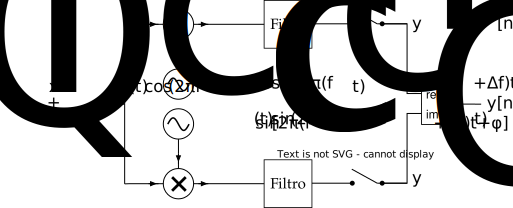
\includegraphics[width=\imsize]{demod-err.pdf}
    \caption{Esquema de demodulador coherente, considerando un error de frecuencia entre la señal entrante y el oscilador local del demodulador.\label{fig:demod-err}}  
\end{figure}

Además, si se contempla que la fase inicial de la señal es desconocida, este error en fase también se manifiesta la señal en banda base de la siguiente forma:
\begin{equation}
    y[n] = x[n] e^{j(2\pi\Delta f T_s n+\phi)}.
\end{equation}
Los algoritmos de sincronismo utilizados en este proyecto son capaces de estimar el desvío en frecuencia de portadora sin ser afectados por el error en fase.


\section{Algoritmos de sincronismo}

En esta sección se describirán dos algoritmos de sincronismo capaces de identificar la muestra inicial de la trama y el desvío de frecuencia de portadora en base al conocimiento de la secuencia de entrenamiento de símbolos cortos. Sus principios de funcionamiento son similares, en su descripción las muestras de la secuencia de entrenamiento de símbolos cortos se agrupan en un vector denotado $\mathbf{s}$, siendo conocida su longitud en muestras, $N$. 

Los métodos definen un estadístico $\Phi$ a partir de las $N$ muestras más recientes de una señal recibida, agrupadas en un vector denominado $\mathbf{y}$. Teniendo $\Phi$ se estimará un instante $\widehat{n}$, que corresponde la muestra en la que se terminó de recibir la secuencia de entrenamiento de símbolos cortos y determina el inicio de la trama. Asociado a esa muestra se obtiene una estimación del desvío de frecuencia de portadora, $\widehat{\Delta f}$. 

\subsection{Banco de correladores}
\label{S:ch3-banco}

Este método se basa en en buscar la forma conocida de la secuencia de entrenamiento de símbolos cortos en la señal recibida, calculando la correlación de $\mathbf{y}$ con señales llamadas referencias construídas a partir de $\mathbf{s}$. 

\subsubsection{Estimación de inicio de trama con una única referencia}

Se desea identificar el instante de inicio de trama, bajo la suposición de que no existe desvío en frecuencia de portadoras. En estas conciciones la función que cumple el objetivo de ser máxima en el instante de interés es simplemente el módulo de la correlación con la secuencia de entrenamiento de símbolos cortos, dada por
\begin{equation}\label{eq:correladores-1}
    \Phi_{BC}[n] = \left\lvert \sum_{k=0}^{N-1}y^\ast[n-k]s[N-k] \right\rvert.
\end{equation}

La aplicación del módulo causa que el error en fase no afecte al estadístico, ya que este es una constante compleja de módulo unitario que sale como factor común de la correlación. Para validar este desempeño, en la Figura \ref{fig:banco-xcorr1} se grafica el resultado de calcular $\Phi_{BC}$ sobre una señal compuesta únicamente por un preámbulo al cual se le ha aplicado un error en fase. se observa que $\Phi_{BC}$ alcanza su valor máximo en la muestra final de la secuencia de entrenamiento de símbolos cortos, por lo tanto $\widehat{n}$ es simplemente la muestra que lo maximiza,
\begin{equation}
    \widehat{n}_{BC} = \argmax_n\Phi_{BC}[n].
\end{equation}

\begin{figure}[t]
    \centering{}\includegraphics[width=\imsizeL]{banco-xcorr1.pdf}
    \caption{Resultado de aplicación del estadístico $\Phi_{BC}$ a una señal recibida que consiste en un preámbulo con error en fase.\label{fig:banco-xcorr1}}  
\end{figure}

\subsubsection{Estimación de desvío de frecuencia de portadora}
\label{Ss:ch3-banco-frecuencias}
El método tal como fue definido es capaz de estimar el inicio de trama, pero aún no es capaz de estimar el desvío de frecuencia de portadora. Si se contempla que $\mathbf{y}$ se ve afectada por un desvío en frecuencia de portadora tal como se modela en la Ecuación 3.3, al evaluar la Ecuación 3.5 se observará una degradación en el máximo de $\Phi_{BC}$, la que depende del factor de fase $T_s\Delta f$ y que se cuantificará definiendo el factor de degradación,
\begin{equation}
    \text{Factor de degradacíon} = \frac{\Phi_{Max}(\Delta f)}{\Phi_{Max}\lvert_{\Delta f = 0}}.
\end{equation}
El factor de degradación en función del factor de rotación de fase se calcula numéricamente y se grafica en la figura \ref{fig:degradacion}.
\begin{figure}[t]
    \centering{}\includegraphics[width=\imsize]{degradacion-err-freq.pdf}
    \caption{Resultado del cálculo numérico del factor de degradación del estadístico $\Phi_{BC}$ en función del factor de rotación de fase.\label{fig:degradacion}}  
\end{figure}


Al tomar en cuenta que un desvío de frecuencia de portadora provoca rotación lineal en fase predecible sobre $y[n]$, el principio utilizado para la estimación con un único correlador se puede extender para estimar $\Delta f$. Se eligen $M$ frecuencias equiespaciadas dentro de un rango de frecuencias $W$ en el que se espera que se encuentre contenido $Delta f$. En particular, $M$ se elige impar, y las frecuenias equiespaciadas se denotan como $Delta f_m$, tal que
\begin{equation}
    \Delta f_m = \frac{mW}{M} \qquad\qquad m \in \left[-\frac{M-1}{2},\,\frac{M-1}{2}\right],
\end{equation}
Luego, para cada $\Delta f_m$, se genera una referencia del preámbulo con la rotación lineal en fase correspondiente a ese error en frecuencia, matemáticamente
\begin{equation}
    r_m[k] = s[k] e^{j2\pi \Delta f_m T_s k}.
\end{equation}

Una manera de determinar el paso entre frecuencias adyancentes para las múltiples referencias, consiste en valerse del factor de degradación, bajo la convención de que el mismo tome el valor de -3 dB, lo que implica que el factor de rotación de fase sea menor a 0,0037, de donde se fijan los valores para $W$ y $M$. Aplicar este criterio considerando $T_{SHORT} = 8 \mu\text{s}$ y FFT de 64 puntos se obtiene que el espaciamiento en frecuencias debe ser de 21 kHz como máximo. En la Figura \ref{fig:references} se visualizan algunas referencias generadas usando este criterio.
\begin{figure}[t]
    \centering{}\includegraphics[width=\imsizeL]{references.pdf}
    \caption{Ejemplos de referencias generadas considerando rotación lineal en fase producto de diferentes errores de frecuencia.\label{fig:references}}  
\end{figure}


Teniendo las múltiples referencias se extiende vectorialmente el estadístico $\Phi_{BC}$ calculado
\begin{equation}\label{eq:correladores-banco}
    \overline{\Phi}_{BC}[n,m] = \left\lvert \sum_{k=1}^{N}y^\ast[n-k]r_m[N-k] \right\rvert
\end{equation}

El resultado de aplicar $\overline{\Phi}_{BC}$ a una señal con rotación lineal en fase visualiza en la figura \ref{fig:banco-xcorrN}. Se observa que los índices $n$ y $m$ que maximizan el estadístico son, respectivamente, la muestra final de la secuencia de entrenamiento de símbolos cortos y el índice de la referencia con $\Delta f_m$ más cercano a $\Delta f$. Estos índices serán $\widehat{n}_{BC}$ y $\widehat{m}_{BC}$, y este último se usará para calcular $\widehat{\Delta f}_{BC}$
\begin{equation}
    \widehat{n}_{BC}, \widehat{m}_{BC} = \argmax_{n,m}\overline{\Phi}_{BC}[n,m] \quad \implies \quad     \widehat{\Delta f}_{BC} = \frac{W}{M} \widehat{m}_{BC}
\end{equation}

\begin{figure}[t]
    \centering{}\includegraphics[width=\imsizeL]{banco-xcorrN.pdf}
    \caption{Resultado de aplicación del estadístico $\overline{\Phi}_{BC}$ a una señal recibida que consiste en un preámbulo con rotación lineal en fase provocado por un desvío de frecuencia de protadora de 21 kHz.\label{fig:banco-xcorrN}}  
\end{figure}


\subsection{Método \textit{delay and correlate}}
\label{S:ch3-dac}

El método \textit{Delay and Correlate}, a diferencia del banco de correladores, no usa la forma de onda explícita de la secuencia de entrenamiento de símbolos cortos para sincronizar, sino que utiliza el conocimiento de su periodicidad. La estrategia se centra en tomar las últimas $N$ muestras de la señal recibida y evaluar si cumplen con la periodicidad esperada de la secuencia de entrenamiento de símbolos cortos. 

\subsubsection{Sincronización en tiempo y frecuencia}
\label{Ss:ch3-dac-principio}

En su versión más simple, este método detecta la periodicidad de la señal comparando la primer mitad del intervalo de las últimas $N$ muestras recibidas con la segunda mitad del mismo, usando el factor de correlación, es decir
\begin{equation}\label{eq:dac-estimator}
    \Phi_{DC}[n] = \sum_{k=0}^{R}y^\ast[n-k]y[n-k-R],
\end{equation}

donde el parámetro $R$ es exáctamente $N/2$ donde $N$ es la longitud del preámbulo. Se puede verificar que el módulo de $\Phi_{DC}$ es máximo cuando las señales correspondientes a los dos intervalos evaluados son idénticas salvo por una rotación relativa en fase. De esta forma $\widehat{n}_{DC}$ nuevamente será la muestra que maximice el estadístico,
\begin{equation}
    \widehat{n}_{DC} = \argmax_n\lvert \Phi_{DC}[n] \lvert.
\end{equation}

A su vez, la fase de $\Phi_{DC}$ contiene información de la diferencia relativa en fase de las señales en cada intervalo, lo que permite estimar el error en frecuencia que provocó esa rotación. La fórmula para estimar el error en frecuencia con este método es la siguiente:+
\begin{equation}\label{eq:freq-est-dac}
    \widehat{\Delta f}_{DC} = \frac{1}{2\pi L T_S}\angle\Phi_{DC}[\widehat{n}_{DC}].
\end{equation}

Los resultados de la aplicación de $\Phi_{DC}$ sobre una señal recibida con rotación lineal en fase se visualizan en la figura \ref{fig:dac-result}.
\begin{figure}[t]
    \centering{}\includegraphics[width=\imsizeL]{delay-and-correlate-result.pdf}
    \caption{Resultado de aplicación del estadístico $\Phi_{DC}$ a una señal recibida que consiste en un preámbulo con error de frecuencia.\label{fig:dac-result}}  
\end{figure}


\subsection{Implementaciones en LabVIEW}
\label{Ss:ch3-labview}

La implementación en LabVIEW de los métodos instancia algoritmos para calcular los estadísticos de sincronismo en determinado instante de muestreo $n$. En estos casos se considera una ventana de evaluación que recibe el nombre de $\mathbf{v}$, y son las últimas $N$ muestras recibidas,
\begin{equation}
    \mathbf{v}[n] = 
    \begin{bmatrix}
        y[N-n+1] &  \cdots & y[n]
    \end{bmatrix}.
\end{equation}
En las expresiones para calcular los estadísticos usando cada método, $\overline{\Phi}_{BC}$ y $\Phi_{DC}$ respectivamente, se omite el índice $n$ ya que este es implícitamente el instante de muestreo en el que se ejecutan las operaciones. 


\subsubsection{Implementación del banco de correladores}

\begin{figure}[t]
    \centering{}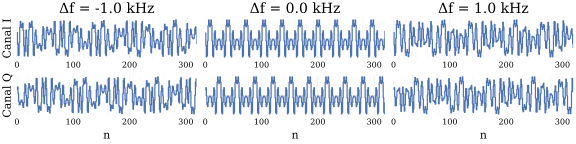
\includegraphics[width=\imsizeL]{xpstopdf/refs.pdf}
    \caption{Diagrama en bloques de las referencias necesarias para calcular el estadístico $\overline{\Phi}_{BC}$ en LabVIEW.\label{fig:refs_lv}}  
\end{figure}

\begin{figure}[t]
    \centering{}\includegraphics[width=\imsize]{xpstopdf/bancox.pdf}
    \caption{Diagrama de bloques del cálculo del estadístico $\overline{\Phi}_{BC}$ en LabVIEW.\label{fig:bancox_lv}}  
\end{figure}

El cálculo del estadístico $\overline{\Phi}_{BC}$ implementado en LabVIEW se ve en el diagrama de bloques presentado en la Figura \ref{fig:bancox_lv}. Requiere de matriz de referencias, llamada $R$, la cual es una matriz de $M \times N$ en donde la fila $m$ son las $N$ muestras de la secuencia de entrenamiento de símbolos cortos con el correspondiente error de frecuencia aplicado,
\begin{equation}
    R_{M\times N} = \begin{bmatrix}
       \cdots & \mathbf{r}_{0} & \cdots\\
       \cdots & \mathbf{r}_{1} & \cdots\\
       & \vdots & \\
       \cdots & \mathbf{r}_{M-1} & \cdots
    \end{bmatrix}.
\end{equation}
Ésta se construye a partir del diagrama de bloques presentado en la Figura \ref{fig:refs_lv}, en el que se toma un rango de errores de frecuencia $W$ y un número de frecuencias $M$, la secuencia de entrenamiento de símbolos cortos $s$ y su duración $T_{SHORT}$. Este diagrama en bloques retorna la matriz de referencias y un vector de errores de frecuencia correspondiente a cada fila de la matriz.

El diagrama de bloques presentado en la Figura \ref{fig:bancox_lv} calcula $\overline{\Phi}_{BC}$ a partir de $R$ y $\mathbf{v}$. Para hacerlo itera sobre las filas de $R$, en cada iteración calculando el factor de correlación de la ventana con la referencia. Esto se consigue con la operación producto interno, y el resultado es un vector de $M$ elementos
\begin{equation}
    \overline{\Phi}_{BC} = \begin{bmatrix}
        \mathbf{v} \cdot \mathbf{r}_{0}\\
        \mathbf{v} \cdot \mathbf{r}_{1}\\
        \vdots\\
        \mathbf{v} \cdot \mathbf{r}_{M-1}
    \end{bmatrix}.
\end{equation}

\subsubsection{Implementación del método \textit{delay and correlate}}

La implementación del método delay and correlate en LabVIEW resulta mucho más simple, su diagrama en bloques se presenta en la Figura \ref{fig:delayx_lv}. El método calcula $L = N/2$ y usa ese valor para particionar $\mathbf{v}$, luego calcula el factor de correlación entre las dos partes por medio del producto interno,
\begin{equation}\textstyle
    \Phi_{DC} = \mathbf{v}_1 \cdot \mathbf{v}_2,
\end{equation}
donde $\mathbf{v}_1$ y $\mathbf{v}_2$ son la primera y la segunda mitad de $\mathbf{v}$ respectivamente.

\begin{figure}[t]
    \centering{}\includegraphics[width=\imsize]{xpstopdf/delayx.pdf}
    \caption{Diagrama de bloques del cálculo del estadístico $\Phi_{DC}$ en LabVIEW.\label{fig:delayx_lv}}  
\end{figure}


\section{Resumen del capítulo}

En este capítulo se definieron los tipos de de error de sincronismo que se deben estimar para la correcta recepción de tramas OFDM: el desvío de temporización de símbolo y el desvío de frecuencia de portadora. 

Se definieron dos métodos que son capaces de realizar un sincronismo inicial tanto en tiempo como en frecuencia, haciendo uso del conocimiento del preámbulo definido en el estándar IEEE 802.11, estos métodos son el banco de correladores y el método de retardo y correlación. Una vez descritos los métodos se ilustró cómo fueron implementados en LabVIEW por medio de diagramas en bloques. 

%%% Local Variables: 
%%% mode: latex
%%% TeX-master: "template"
%%% End: 

\chapter{Algoritmo de detección}
\label{Ch:4}
\graphicspath{{figs/}}
%%%%%%%%%%%%%%%%%%%%%%%%%%%%%%%%%%%%%%%%%%%%%%%%%%%%%%%%%%%%%%%%%%%%%%%%

En este capítulo se trata el problema de detección, el cual es fundamental resolver para el funcionamiento de los algoritmos de sincronismo implementados. La correcta detección de una señal entrante indica en qué instante uno debe invocar los algoritmos de sincronismo definidos e implementados en el Capítulo \ref{Ch:3}. 

La primera parte de este capítulo se centra en la formalización de una prueba de hipótesis que determinará si un registro de datos bajo prueba contiene una señal de interés. Se estudian las propiedades estadísticas del ruido y de una señal afectada por el mismo, y en función de estas propiedades se formaliza una regla de decisión. En la segunda parte se trata el problema de la estimación de la varianza del ruido, ya que conocerla es necesario para la correcta aplicación de la regla de decisión definida.

\section{Prueba de hipótesis}
\label{S:prueba-hipotesis}

El problema de detección se resolverá por medio de una prueba de hipótesis sobre las muestras de una señal presentes en una ventana de recepción, agrupadas en el vector
\begin{equation}\label{eq:def_y}
    \mathbf{y} = \begin{bmatrix}
        y[0] & y[1] & \cdots & y[N-1],
    \end{bmatrix}
\end{equation}
donde $N$ coincide con la longitud de la secuencia de entrenamiento de símbolos cortos. 

Los pasos para realizar la prueba son los siguientes:
\begin{enumerate}
    \item definición de dos o más hipótesis mutuamente excluyentes acerca del origen de las muestras observadas;
    \item definición de un estadístico en función de las muestras bajo estudio, que recibe el nombre $\phi\left[\mathbf{y}\right]$;
    \item definición de una regla de decisión sobre el estadístico elegido para discriminar entre las hipótesis disponibles según determinado criterio;
    \item estimación de los parámetros necesarios para aplicar la regla de decisión;
\end{enumerate}

\subsection{Definición de hipótesis}
\label{Ss:def-hipotesis}

Se definen dos hipótesis sobre la composición de las muestras, estas reciben el nombre de hipótesis nula ($H_0$) e hipótesis alternativa ($H_1$), y son las siguientes:
\begin{itemize}
    \item $H_0$: el intervalo de evaluación contiene únicamente ruido;
    \item $H_1$: el intervalo de evaluación contiene una secuencia de entrenamiento de símbolos cortos afectada por ruido aditivo y modificada por el canal inalámbrico.
\end{itemize}

Se hacen varias suposiciones en las definiciónes de las hipótesis:
\begin{itemize}
    \item las muestras de ruido siguen la distribución normal compleja, son independientes, e idénticamente distribuidas;
    \item la respuesta al impulso del canal puede ser aproximada por un único \textit{tap}, por lo que cada muestra de la secuencia transmitida se ve modificada por un factor de amplitud y fase, pero no influye a las muestras anteriores ni a las siguientes;
    \item el canal presenta desvanecimiento lento, por lo que el factor que modifica la amplitud y fase de una señal recibida se mantiene aproximadamente constante.
\end{itemize}

Tomando en cuenta las suposiciones, se procede a formalizar las expresiones matemáticas de las hipótesis;
\begin{equation}\label{eq:def-hipótesis}
    \begin{aligned}
        H_0&: \quad \mathbf{y} = \mathbf{w}\\
        H_1&: \quad \mathbf{y} = A\mathbf{s} + \mathbf{w}
    \end{aligned}
    \qquad\qquad
    \mathbf{w} \sim \mathcal{CN}\left[\mathbf{0},\, \sigma^2 I_N\right],
\end{equation}
donde $\mathbf{s}$ es la secuencia de entrenamiento de símbolos cortos, de $N$ muestras de longitud, y $A$ es un factor complejo desconocido, pero constante, que modifica la amplitud y fase de la secuencia. 

\subsubsection{Definición de SNR}
\label{Ss:def-snr}

En el caso de que la hipótesis alternativa sea verdadera, resulta conveniente definir una medida de la relación señal a ruido. La definición utilizada es el cociente entre la potencia media de una muestra de señal y la potencia media de una muestra de ruido
\begin{equation}\label{eq:snr-definicion}
\text{SNR} = \frac{\text{Potencia media señal}}{\text{Potencia media ruido}}.
\end{equation}

Las suposiciones hechas implican que la potencia media de la señal es un valor determinístico, dado por
\begin{equation}\label{eq:potencia-señal}
\overline{P}_s = \frac{1}{N}\sum_{k=0}^{N-1}\lvert A s[k] \rvert^2 = \frac{1}{N} \lvert A \rvert^2 \lVert \mathbf{s} \rVert^2,
\end{equation}
mientras que la potencia media del ruido surge de las propiedades estadísticas de su distribución, y se calcula a partir de la propiedad del módulo de una variable aleatoria normal compleja, el cual sigue una distribución Rayleigh
\begin{equation}
w[k] \sim \mathcal{CN}\left[0, \sigma^2\right]  \implies|w[k]| \sim \mathcal{R}ay\left[\sigma\right],
\end{equation}
y el hecho de que media de la distribución Rayleigh es conocida, así como lo es su varianza
\begin{equation}
E\left[\lvert w[k]\rvert\right] = \sigma \sqrt{\frac{\pi}{2}}\qquad\qquad V[\left\lvert w[k] \rvert\right] = \frac{4-\pi}{2} \sigma^2,
\end{equation}
lo cual permite calcular la potencia media de una muestra de ruido de la siguiente forma
\begin{equation}\label{eq:potencia-ruido}
    E\left[\lvert w[k]\rvert^2\right] = V\left[\lvert w[k]\rvert\right] + E\left[\lvert w[k]\rvert\right]^2 =  2\sigma^2.
\end{equation}

Remplazando los valores obtenidos de las Ecuaciones \ref{eq:potencia-señal} y \ref{eq:potencia-ruido} en la Ecuación \ref{eq:snr-definicion} se obtiene la expresión de la SNR presente cuando la hipótesis alternativa es verdadera,
\begin{equation}
\text{SNR} = \frac{\lvert A\rvert^2 \lVert \mathbf{s} \rVert ^2}{2N \sigma^2}.
\end{equation}

\subsection{Elección de estadístico de detección}
\label{Ss:hipotesis-estadistico}


El estadístico utilizado será el mismo que se calcula en el algoritmo de sincronismo con banco de correladores, ésto es la correlación con la secuencia de entrenamiento de símbolos cortos. Por practicidad se expresará de la siguiente forma
\begin{equation}
    \phi[\mathbf{y}] = \left\lvert\sum_{k=0}^N s^\ast[k]y[k]\right\rvert = \lvert \mathbf{s}^\ast\mathbf{y}\rvert.
\end{equation}

Al momento de estudiar las propiedades estadísticas de $\phi$ resulta conveniente trabajar con un resultado intermedio, el cual es el valor complejo de la correlación previo a la operación módulo,
\begin{equation}
    \psi[\mathbf{y}] = \sum_{k=0}^N s^\ast[k]y[k] = \mathbf{s}^\ast\mathbf{y}.
\end{equation}

\subsection{Distribución del estadístico ante hipótesis nula}

Se estudia la distribución del estadístico $\psi$ en el caso que $\mathbf{y}$ posee únicamente la contribución del ruido,
\begin{equation}\label{eq:psi-ante-h0}
    \mathbf{y} | H_0 = \mathbf{w} \implies \psi[\mathbf{y}] | H_0= \sum_{k = 0}^{N-1} s^\ast[k]w[k].
\end{equation}

En estas condiciones, se observa que $\psi$ resulta una sumatoria de muestras de ruido, cada muestra escalada por su correspondiente término de la secuencia de entrenamiento de símbolos cortos. Esto resulta en una sumatoria de variables normales complejas independientes de diferente varianza. La distribución de cada término de la sumatoria, $z[k] = s^\ast[k]w[k]$, es la siguiente:
\begin{equation}
    z[k] \sim \mathcal{CN}[0,\, \lvert s[k]\rvert^2\sigma^2].
\end{equation}

A partir de la distribución de los términos, distribución de la sumatoria se calcula con las propiedades de la suma de variables aleatorias gaussianas independientes, y se reduce a la siguiente expresión:
\begin{equation}
    \begin{aligned}
        \psi | H_0 &\sim \mathcal{CN}\left[0,\, \sum_{k=0}^{N-1} \lvert s[k]\rvert^2  \sigma^2 \right],\\[0.5em]
        \psi | H_0 &\sim \mathcal{CN}\left[0,\,\lVert \mathbf{s}\rVert^2  \sigma^2 \right].
    \end{aligned}
\end{equation}

Al igual que se ha visto en la Sección \ref{Ss:def-snr}, el módulo de una distribución normal compleja sigue una distribución Rayleigh, por lo que se conoce la distribución de $\phi$ condicionada por $H_0$. La expresión de su distribución acumulada resulta
\begin{equation}\label{eq:phi-ante-h0}
    F_\phi(\phi|H_0) = 1- \exp\left[-\frac{\phi^2}{2\lVert\mathbf{s}\rVert^2 \sigma^2}\right].
\end{equation}

\subsection{Distribución del estadístico ante hipótesis alternativa}

Nuevamente, se parte de la distribución de $\psi$, en este caso cuando la hipótesis alternativa es verdadera,
\begin{equation}\label{eq:psi-ante-h1}
    \begin{aligned} 
        \mathbf{y} | H_! = A\mathbf{s} + \mathbf{w} \implies \psi[\mathbf{y}] | H_1  
        &= \mathbf{s}^\ast\left(A\mathbf{s}+\mathbf{w}\right)\\ 
        &= A\lVert\mathbf{s}\rVert^2+\mathbf{s}^\ast\mathbf{w}.
    \end{aligned}
\end{equation}

Es evidente la similitud de este caso con el estudiado anteriormente. La Ecuación \ref{eq:psi-ante-h1} describe la suma de un término determinístico y un término aleatorio, el efecto del término determinístico es únicamente el de desplazar la media de la distribución, obteniendo
\begin{equation}
    \psi | H_1 \sim \mathcal{CN}\left[A\lVert\mathbf{s}\rVert^2,\,\lVert \mathbf{s}\rVert^2  \sigma^2 \right].
\end{equation}

Nuevamente, $\psi$ sigue una distribución normal compleja, pero en este caso ya no es de media nula. Para proceder se normaliza la variable aleatoria, definiendo una nueva variable aleatoria $\psi'$ con varianza unitaria,
\begin{equation}
    \psi' = \frac{\psi}{\lVert \mathbf{s} \rVert \sigma} \quad \implies \quad     \psi' | H_1 \sim \mathcal{CN}\left[\frac{A\lVert\mathbf{s}\rVert}{\sigma},\, 2 \right],
\end{equation}
y con el mismo factor de normalización se define la variable $\phi'$, la cual comparte con $\psi'$ la misma relación que sus respectivas equivalentes no normalizadas:
\begin{equation}
\phi' = \frac{\phi}{\lVert \mathbf{s} \rVert \sigma} \quad \longrightarrow \quad     \phi' = \lvert\psi'\rvert.
\end{equation}

El propósito de la normalización es que ésta permite utilizar la definición de la distribución $\chi$ no central \cite{distributions}, la cual es definida de la siguiente forma: si existen $n$ variables aleatorias normales $x_i$ independientes de varianza unitaria y respectivas medias $\mu_i$, y se define $z$ como la raíz de la sumatoria de sus cuadrados
\begin{equation}
    z = \sqrt{\sum_{i=1}^{n}x_i^2},
\end{equation}
ésta variable seguirá la distribución $\chi$ no central de $n$ grados de libertad y parámetro de no-centralidad $\lambda$, el cual es calculado de la siguiente forma
\begin{equation}
    \lambda = \sqrt{\sum_{i=1}^{n}\mu_i^2}.
\end{equation}

Esta definición permite encontrar la distribución de $\phi'$, en tal caso se tiene $n = 2$ grados de libertad, $x_1$ y $x_2$ son la parte real e imaginaria de $\psi'$ respectivamente, y $\mu_1$ y $\mu_2$ son la parte real e imaginaria de su media compleja. Se obtiene el parámetro $\lambda$
\begin{equation}
    \displaystyle\mu_1 = \frac{\rVert\mathbf{s}\rVert}{\sigma}\mathcal{R}e\left[A\right] \quad \displaystyle\mu_2 = \frac{\rVert\mathbf{s}\rVert}{\sigma}\mathcal{I}m\left[A\right] \quad \implies \quad \lambda = \frac{\lVert\mathbf{s}\rVert}{\sigma}\lvert A \rvert
\end{equation}

Resulta la distribución
\begin{equation}
    \phi' | H_1 \sim \chi_{NC}\left[n = 2, \, \lambda = \frac{|A|\lVert\mathbf{s}\rVert}{\sigma}\right] 
\end{equation}

Tal como se hizo en el caso anterior, se continúa trabajando con la función de probabilidad acumulada, la cual en esta oportunidad está dada por
\begin{equation}
    F_{\phi'}(\phi'|H_1) = 1-\int_{\phi'}^\infty x\exp\left[-\frac{x^2 + \frac{|A|^2\lVert\mathbf{s}\rVert^2}{\sigma^2}}{2}\right]I_0\left[\frac{|A|\lVert\mathbf{s}\rVert}{\sigma} x\right] dx,
\end{equation}
en donde $I_n[z]$ es la función de Bessel modificada de primera especie. 

Finalmente, se aplica el cambio de variables para revertir la normalización, obteniendo la distribución acumulada de $\phi$ condicionada por la hipótesis alternativa
\begin{equation}\label{eq:phi-ante-h1}
    F_\phi(\phi|H_1) = 1-\int_{\frac{\phi}{\lVert\mathbf{s}\rVert\sigma}}^\infty x\exp\left[-\frac{x^2 + \frac{|A|^2\lVert\mathbf{s}\rVert^2}{\sigma^2}}{2}\right]I_0\left[\frac{|A|\lVert\mathbf{s}\rVert}{\sigma} x\right] dx.
\end{equation}


\subsection{Regla de decisión}
\label{Ss:hipotesis-umbral}\label{eq:def-pfa}

La regla de decisión típica en los casos que se cuentan con dos hipótesis es la comparación del estadístico con un umbral $T$, tal que si el estadístico excede el umbral se decide por la hipótesis alternativa, mientras que si no lo hace se opta por la hipótesis nula,
\begin{equation}
    \phi[\mathbf{y}]\mathop{\lessgtr}_{H_1}^{H_0}T.
\end{equation}

En función del estadístico y el umbral se definen la probabilidad de falsa alarma, $P_{FA},$, que es la probabilidad de decidir por la hipótesis alternativa cuando la hipótesis nula es verdadera
\begin{equation}
    P_{FA} = \int_T^\infty f_\phi(\phi|H_0)d\phi = 1 - F_\phi(T|H_0).
\end{equation}

Asimismo, se define la probabilidad de Detección, $P_D$, la cual es la probabilidad de decidir por la hipótesis alternativa cuando esta efectivamente es verdadera
\begin{equation}\label{eq:probabilidad-deteccion-def}
    P_{D} = \int_T^\infty f_\phi(\phi|H_1)d\phi = 1 - F_\phi(T|H_1)
\end{equation}

El criterio elegido para la elección del umbral es tal que la probabilidad de falsa alarma se mantenga constante a un valor elegido. Tomando la expresión de $F_\phi(\phi|H_0)$ calculado en la Ecuación \ref{eq:phi-ante-h0}, y remplazándolo en la Ecuación \ref{eq:def-pfa} se obtiene
\begin{equation}
    P_{FA} = \exp\left[-\frac{T^2}{2\lVert\mathbf{s}\rVert^2 \sigma^2}\right],    
\end{equation}
y despejando $T$ surge la función para determinar el umbral que obtendrá la probabilidad de falsa alarma deseada
\begin{equation}\label{eq:umbral}
    T(P_{FA}) = \sqrt{-2\lVert \mathbf{s}\rVert^2 \sigma^2 \ln\left[P_{FA}\right]}    ,
\end{equation}

\begin{figure}[t]
    \centering{}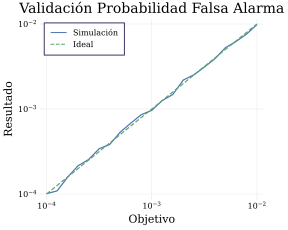
\includegraphics[width=\imsize]{pfa_test.pdf}
    \caption{Resultados de simulación para verificar la correcta probabilidad de falsa alarma de la regla de decisión.\label{fig:pfa-test}}  
\end{figure}

El correcto funcionamiento del umbral para el criterio elegido se verifica por medio de una simulación, la cual consiste en ejecutar los siguientes pasos:
\begin{enumerate}
    \item se fijan los valores de $P_{FA}$ y $\sigma^2$ y se calcula el valor de $T$ a partir de ellos;
    \item para tener un número de realizaciones razonables pero estadísticamente representativo del experimento, se elige hacer $100/P_{FA}$ realizaciones;
    \item para cada realización se genera un vector $\mathbf{y}$ de $N$ muestras de ruido normal complejo con la varianza elegida; 
    \item se calcula $\phi[\mathbf{y}]$ y se compara el resultado con el valor de $T$, registrando si se produce o no una falsa alarma;
    \item una vez terminadas las realizaciones, la probabilidad de falsa alarma empírica es el número de falsas alarmas dividido por el número total de realizaciones.
\end{enumerate}
La simulación verifica que la regla de decisión efectivamente alcanza la probabilidad de falsa alarma deseada. Los resultados de la misma se presentan en la Figura \ref{fig:pfa-test}.

\subsection{Desempeño de la regla de decisión}
\label{Ss:hipotesis-desempeño}
El desempeño de la regla de decisión se evalúa estudiando cómo se verá afectada la probabilidad de detección en función de los demás parámetros. La probabilidad de detección se conoce al tomar la Ecuación \ref{eq:probabilidad-deteccion-def} y reemplazar $F_\phi(\phi|H_1)$ calculado en la Ecuación \ref{eq:phi-ante-h1} y el valor del umbral calculado en la Ecuación \ref{eq:umbral}
\begin{equation}\label{eq:probabilidad-deteccion}
    P_D = \int_{\sqrt{-2 \ln\left[P_{FA}\right]}}^\infty x\exp\left[-\frac{x^2 + \frac{|A|^2\lVert\mathbf{s}\rVert^2}{\sigma^2}}{2}\right]I_0\left[\frac{|A|\lVert\mathbf{s}\rVert}{\sigma} x\right] dx.
\end{equation}

Al observar la expresión de la probabilidad de detección resultante, se nota que tanto $A$ como $\sigma$ solo influyen en esta a través de la relación entre estos, lo cual es un resultado razonable. Esto incentiva a expresar la probabilidad de detección en función de la SNR, expresada en la Ecuación \ref{eq:snr-definicion}.
\begin{equation}\label{eq:probabilidad-deteccion-snr}
    P_D = \int_{\sqrt{-2 \ln\left[P_{FA}\right]}}^\infty x\exp\left[-\frac{x^2 + 2N\,\text{SNR}}{2}\right]I_0\left[\sqrt{2N\,\text{SNR}}\,x\right] dx
\end{equation}

\begin{figure}[t]
    \centering{}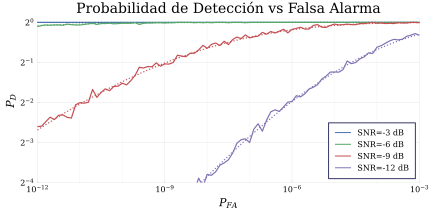
\includegraphics[width=\imsize]{pd_vs_pfa.pdf}
    \caption{Resultados de probabilidad de detección de la decisión en función de la probabilidad de falsa alarma elegida a valores de SNR fijos. En línea punteada se grafican los resultados analíticos, y en línea contínua del mismo color los resultados de simulación.\label{fig:pd-vs-pfa}}
\end{figure}
\begin{figure}[t]
    \centering{}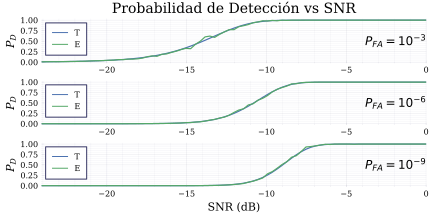
\includegraphics[width=\imsize]{pd_vs_snr.pdf}
    \caption{Resultados de probabilidad de detección de la decisión en función de la SNR elegida a valores de probabilidad de falsa alarma elegida fijos. En línea punteada se grafican los resultados analíticos, y en línea contínua del mismo color los resultados de simulación.\label{fig:pd-vs-snr}}  
\end{figure}


Al expresarlo así se nota que la probabilidad de detección depende de la probabilidad de falsa alarma elegida y de la relación señal a ruido presente en la señal. De esa dependencia se pueden evaluar dos medidas de desempeño, la probabilidad de detección en función de la probabilidad de error a SNR constante y la probabilidad de detección en función de la SNR a probabilidad de falsa alarma constante. Estas métricas de desempeño se validan con simulaciones numéricas, las cuales se realizan de la siguiente forma:
\begin{enumerate}
    \item se fijan los valores de $P_{FA}$ y SNR, se determinan arbitrariamente valores de $A$ y $\sigma^2$ que resulten en la SNR elegida al aplicar la Ecuación \ref{eq:snr-definicion}, y se calcula el valor de $T$;
    \item para tener un número de realizaciones razonable, pero estadísticamente representativo del experimento, se elige hacer $100/P_D$ realizaciones;
    \item en cada realización se genera un vector de $N$ muestras $\mathbf{y} = A\mathbf{s}+\mathbf{w}$ con los valores de $A$ y $\sigma^2$ elegidos anteriormente;
    \item se calcula $\phi[\mathbf{y}]$ y se compara el resultado con el valor de $T$, registrando si se produce o no una detección;
    \item una vez terminadas las realizaciones, la probabilidad de detección empírica es el número de detecciones dividido por el número total de realizaciones.
\end{enumerate}

Estas simulaciones se ejecutan sobre un vector de valores de SNR manteniendo un valor de $P_{FA}$ fijo, y sobre un vector de valores de $P_{FA}$ manteniendo un valor de SNR fijo. Los resultados de $P_D$ empírico se comparan con las curvas que resultan de evaluar la Ecuación \ref{eq:probabilidad-deteccion-snr}, y se muestran en las Figuras \ref{fig:pd-vs-snr} y \ref{fig:pd-vs-pfa} respectivamente. 

\section{Estimación de varianza del ruido}
\label{S:estimacion-ruido}

El problema de detección se definió en función de un umbral el cual depende de la varianza del ruido, tal como se muestra en la Ecuación \ref{eq:umbral} que este depende de la varianza del ruido. Sin embargo, la varianza del ruido es desconocida, y ésta necesita estimarse para poder calcular el umbral. 

Existen varios criterios para elegir un estimador adecuado para el problema, en este caso se elige el estimador insesgado de mínima varianza (MVUE por sus siglas en inglés). Se supone que la estimación del ruido se realiza sobre un vector de muestras que proviene únicamente del ruido, caso que corresponde a la hipótesis nula de la regla de decisión.

\subsection{Cálculo del MVUE de varianza del ruido}
% Para estimar la varianza del ruido, se selecciona el estimador insesgado de mínima varianza (MVUE por sus siglas en inglés). El método para encontrarlo es usando el teorema de Rao-Blackwell-Lehmann-Scheffe. \cite{kay}
% 
% El procedimiento requiere de un estadístico suficiente para un parámetro de la distribución de ciertos datos obtenidos. 
% Los datos se suponen provenientes de ruido normal complejo de media nula independientes e idénticamente distribuidos, se le asigna el nombre $\mathbf{w}$ y su distribución será la siguiente. 
% \begin{equation}\label{eq:noise-estimation-distribution}
%     f(\mathbf{w}) = \frac{1}{\left(2\pi\sigma^2\right)^N} \exp\left[- \frac{\mathbf{w}^\ast \mathbf{w}}{2\sigma^2}\right]
% \end{equation}
% 
% El teorema establece que si uno encuentra una función de un estadístico suficiente que retorne un estimador insesgado del parámetro, este será el MVUE. 
% 
% Para obtener el estadístico suficiente, se utiliza el teorema de factorización de Neyman--Fischer establece que si la distribución de probabilidad de $\mathbf{w}$ puede ser expresada como el producto
% \begin{equation}
%     f(\mathbf{w}, \sigma^2) = g(T(\mathbf{w}), \sigma^2)h(\mathbf{w})
% \end{equation}
% 
% Entonces $T(\mathbf{w})$ es un estadístico suficiente para $\sigma^2$. Efectivamente la distribución tal como es descrita en la ecuación \ref{eq:noise-estimation-distribution} tiene esta forma si se eligen las siguientes funciones
% \begin{equation}
%     h(\mathbf{w}) = 1 \qquad\qquad T(\mathbf{w}) = \mathbf{w}^\ast \mathbf{w}
% \end{equation}
% 
% Para obtener una función de $T(\mathbf{w})$ que retorne un estimador insesgado, resulta util calcular el valor esperado de $T(\mathbf{w})$, lo cual en este caso es fácil ya que las muestras son independientes e idénticamente distribuidas. 
% \begin{equation}
%     E\left[\mathbf{w}^\ast\mathbf{w}\right] =  E\left[\sum_{i=0}^{N-1}\lvert w[i]\rvert^2\right]  =   \sum_{i=0}^{N-1}E\left[\lvert w[i]\rvert^2\right] 
% \end{equation}
% 
% El valor esperado del módulo al cuadrado de una muestra de ruido fue calculado anteriormente, en la Sección \ref{Ss:def-hipotesis}. De esta forma se obtiene el siguiente valor
% \begin{equation}
%     E\left[\mathbf{w}^\ast\mathbf{w}\right] =  \sum_{i=0}^{N-1}2\sigma^2 = 2N\sigma^2 
% \end{equation}
% 
% Conociendo ese valor, puede calcular facilmente una función que retorne un estadístico insesgado aplicando un factor de correción multiplicativo, esta función será el MVUE.
% \begin{equation}
%     \widehat{\sigma^2}_{\text{MVU}} = g\left(\mathbf{w}^\ast\mathbf{w}\right) =  \frac{\mathbf{w}^\ast\mathbf{w}}{2N}
% \end{equation}

El MVUE se puede encontrar utilizando el teorema de la cota inferior de Cramer-Rao \cite{kay}, la cual establece que si la distribución de probabilidad de una variable $\mathbf{x}$ afectada por un parámetro $\theta$ cumple la condición de regularidad
\begin{equation}
    E\left[\frac{\partial \ln p(\mathbf{x},\theta)}{\partial \theta}\right] = 0,
\end{equation}
y la derivada respecto al parámetro del logaritmo de la distribución de probabilidad de la variable aleatoria se puede factorizar de la siguiente forma
\begin{equation}\label{eq:cramer-rao}
    \frac{\partial \ln p(\mathbf{x},\theta)}{\partial \theta} = I(\theta)\left(g(\mathbf{x})-\theta\right),
\end{equation}
entonces $g(\mathbf{x})$ será el MVUE para $\theta$. Además, $I(\theta)$ será la información de Fisher de este parámetro, y ésta es inversamente proporcional a la varianza del MVUE,
\begin{equation}\label{eq:var-mvue}
    \text{Var}[\widehat{\theta}_{\text{MVU}}] = \frac{1}{I(\theta)}.
\end{equation}

En este caso el parámetro a estimar es la varianza a partir de un vector de muestras de ruido $\mathbf{w}$, por lo cual $\theta = \sigma^2$, y la distribución de probabilidad de $\mathbf{w}$ queda representada de la siguiente forma 
\begin{equation}\label{eq:noise-estimation-distribution}
    f(\mathbf{w}, \theta) = \frac{1}{\left(2\pi\theta\right)^N} \exp\left[- \frac{\mathbf{w}^\ast \mathbf{w}}{2\theta}\right],
\end{equation}
en base a la cual se procede a calcular la derivada respecto al parámetro del logaritmo de la distribución de las muestras, obteniendo la expresión
\begin{equation}\label{eq:logaritmo-derivada}
\frac{\partial \ln p(\mathbf{w},\theta)}{\partial \theta} =  - \frac{N}{ \theta} +\frac{\mathbf{w}^\ast\mathbf{w}}{2\theta^2}
\end{equation}

La condición de regularidad se puede verificar fácilmente, al considerar que las muestras son independientes e idénticamnte distribuidas. A su vez, la Ecuación \ref{eq:logaritmo-derivada} se puede factorizar de la siguiente forma;
\begin{equation}\label{eq:logaritmo-derivada-factorizacion}
    \frac{\partial \ln p(\mathbf{w},\theta)}{\partial \theta} =  \frac{N}{\theta^2}\left(\frac{\mathbf{w}^\ast\mathbf{w}}{2N}-\theta\right),
\end{equation}
la cual es consistente con la Ecuación \ref{eq:cramer-rao}, y nos da el MVUE y la información de Fisher;
\begin{equation}\label{eq:expresion-mvue}
    \widehat{\sigma^2}_{\text{MVU}} = \frac{\mathbf{w}^\ast\mathbf{w}}{2N} \qquad\qquad I(\sigma^2) = \frac{N}{\left(\sigma^2\right)^2}
\end{equation}
% El valor esperado del módulo al cuadrado de una muestra de ruido fue calculado anteriormente, en la Sección \ref{Ss:def-hipotesis}. De esta forma se obtiene el siguiente valor
% \begin{equation}
%     E\left[\mathbf{w}^\ast\mathbf{w}\right] =  \sum_{i=0}^{N-1}2\sigma^2 = 2N\sigma^2 
% \end{equation}

\subsection{Desempeño del estimador}
\label{Ss:estimador-ruido-desempeño}

%\begin{equation}  
%    \begin{aligned}
%        \ln p(\mathbf{w},\sigma^2) &= - N \ln\left[2\pi \sigma^2\right]-\frac{\mathbf{w}^\ast\mathbf{w}}{2\sigma^2}\\
%        \frac{\partial \ln p(\mathbf{w},\sigma^2)}{\partial \sigma^2} &=  - \frac{N}{ \sigma^2} +\frac{\mathbf{w}^\ast\mathbf{w}}{2\left(\sigma^2\right)^2}\\
%        \frac{\partial^2 \ln p(\mathbf{w},\sigma^2)}{\partial \left(\sigma^2\right)^2} &=   \frac{N}{\left(\sigma^2\right)^2}-  \frac{\mathbf{w}^\ast\mathbf{w}}{\left(\sigma^2\right)^3}
%    \end{aligned}
%\end{equation}
 
La métrica utilizada para evaluar el desempeño del estimador será el error cuadrático medio, definido de la siguiente forma
\begin{equation}
    \text{MSE}[\widehat{\theta}] = E\left[(\widehat{\theta}-\theta)^2\right] = \text{Var}[\widehat{\theta}] + b^2[\widehat{\theta}],
\end{equation}
donde $b[\widehat{\theta}]$ es el sesgo del estimador. En el caso de los estimadores insesgados como lo es el MVUE, el error cuadrático medio es igual a la varianza del estimador. La varianza del MVUE fue calculada teóricamente a partir de la cota inferior de Cramer-Rao y se Ecuación \ref{eq:var-mvue}, por lo que el error cuadrático medio teórico del estimador es conocido
\begin{equation}\label{eq:mvue-mse}
    \text{MSE}[\widehat{\sigma^2}_{\text{MVU}}] = \frac{\left(\sigma^2\right)^2}{N}.
\end{equation}
El desempeño del MVUE se valida calculando el error cuadrático del mismo sobre realizaciones de ruido con varianza conocida, y se verifica que éste tenga el comportamiento esperado. Este resultado se presenta en la Figura \ref{fig:estimator_mse}.
\begin{figure}[t]
    \centering{}\includegraphics[width=\imsize]{estimator_mse.pdf}
    \caption{Resultados de la verificación por simulación del error cuadrático medio del MVUE para la varianza del ruido.\label{fig:estimator_mse}}
\end{figure}

En principio, se podría estimar el ruido a partir de las mismas muestras que se utilizan para calcular $\phi$. Sin embargo, estas muestras no siempre van a cumplir la supocisiones que se planetaron para derivar la expresión del MVUE, las cuales implicaban que la hipótesis nula es verdadera. Se procede a evaluar numéricamente si el error cuadrático medio del estimador incrementa al aplicar el mismo ante la hipótesis alternativa. 

Ese ensayo se logra generando múltiples realizaciones de un vector $\mathbf{y}$ que consistan en una secuencia de entrenamiento de símbolos cortos más ruido con determinada SNR, calculando el MVUE expresado en la Ecuación \ref{eq:expresion-mvue} en en esas condiciones, y promediando el error cuadrático. Los resultados se muestran en la Figura \ref{fig:estimator_mse_snr} 
\begin{figure}[t]
    \centering{}\includegraphics[width=\imsize]{estimator_mse_snr.pdf}
    \caption{Resultados de simulación numérica del cálculo del error cuadrático medio normalizado del MVUE para la varianza del ruido ante la presencia de una secuencia de entrenamiento de símbolos cortos con determinada SNR en la ventana de muestras utilizadas para calcular el estadístico.\label{fig:estimator_mse_snr}}
\end{figure}

Se observa que la estimación del ruido será incorrecta cuando la hipótesis alternativa sea verdadera, este fenómeno afectaría el cálculo del umbral si no se tomara en cuenta. La estrategia para evitar este efecto es simple cuando se consideran las propiedades de la transmisión. Se sabe que el preámbulo se recibe al inicio de cualquier señal OFDM, previo a éste no existe señal. Teniendo en cuenta esto, basta utilizar muestras pasadas para estimar el ruido y calcular el umbral contra el cual se comparará el estadístico de detección actual para la regla de decisión.

\section{Resumen del capítulo}

Se formalizaron las hipótesis mutuamente excluyentes acerca de la composición de las muestras de la señal recibida: una hipótesis nula que corresponde a la ausencia de una señal entrante; y una hipótesis alternativa que corresponde a la presencia de la misma. En el caso de que exista una señal entrante, se definió una medida de relación señal a ruido.  

En función de las muestras recibidas se definió un estadístico y una regla de decisión en base a un umbral contra el cual se compara el estadístico elegido para discriminar entre las hipótesis. Se definieron la probabilidad de detección y la probabilidad de falsa alarma, ésta última se usó para elegir el valor del umbral, y se analizó cómo la probabilidad de falsa alarma elegida y la SNR afectan a la probabilidad de detección. 

Finalmente, se encontró el estimador insesgado de mínima varianza para la varianza del ruido, el cual será necesario para definir el umbral de la regla de decisión. Se observó que la presencia de señales en las muestras recibidas afecta el desempeño de este estimador, por lo que se propone resolver este problema por medio de un desfasaje temporal en la ventana que se utiliza para estimar la varianza del ruido y la ventana sobre la cual se aplica la regla de decisión.
\chapter{Implementación de algoritmos de detección y sincronismo en SDR}
\label{Ch:5}
\graphicspath{{figs/}}

En los Capítulo \ref{Ch:3} y \ref{Ch:4} se detallaron de forma independiente los algoritmos de sincronismo y detección, respectivamente, aplicables a señales que emplean OFDM en el estándar IEEE 802.11. En este capítulo se detallará la integración de dichos algoritmos en un sistema desarrollado en LabVIEW capaz de operar de forma contínua, con la función de detectar la presencia de señales transmitidas de acuerdo al estándar en las muestras adquiridas por un receptor y estimar los parámetros de sincronismo correspondientes a cada señal detectada. 

El desarrollo del sistema a diseñar contempló varias etapas. En la primera etapa se implementó un entorno de simulación del problema sobre el cual se verificó el funcionamiento del mismo con señales generadas internamente consistentes con las suposiciones hechas durante las derivaciones de los algoritmos correspondientes. En la siguiente etapa se evaluó la factibilidad de utilizar el sistema diseñado sobre señales reales adquiridas por un dispositivo periférico de radio universal programable del fabricante National Instruments NI USRP-2953R, utilizando la USRP únicamente para adquisición de muestras y realizando el procesamiento en el \textit{host}. Finalmente, se analizaron las limitaciones de este método y se consideró la necesidad de transferir una o más etapas de procesamiento a la USRP por medio del diseño de componentes FPGA personalizados.

\section{Diseño general del sistema}
\label{S:ch5-general}

\begin{figure}[t]
    \centering{}\includegraphics[width=\imsizeL]{xpstopdf/top_level.pdf}
    \caption{Diagrama de bloques \textit{top-level} del sistema que integra los algoritmos de detección y sincronismo en ejecución contínua sobre las muestras de una señal recibida implementado en LabVIEW, utilizando una simulación del problema como fuente de muestras.\label{fig:top-level-lv}}  
\end{figure}

La implementación de los algoritmos de detección y sincronismo en LabVIEW contempla una etapa de inicialización seguida de un ciclo \textit{while} que se ejecutará contínuamente. En cada iteración del ciclo \textit{while} se toma una muestra proveniente de una fuente y se registra en memoria, luego se ejecutan varias etapas secuenciales de procesamiento, y finalmente se actualiza un registro de detecciones y sus correspondientes estimaciones referentes al sincronismo. La esquemática \textit{top-level} del diseño se presenta en la Figura \ref{fig:top-level-lv}.

En un entorno de simulación, la tasa de iteraciones del ciclo \textit{while} puede ser arbitraria, pero para que el diseño implementado sea capaz de operar en tiempo real la tasa de iteraciones debe ser igual a la tasa de muestreo que tendrá el receptor. La tasa de muestreo depende del espaciamiento entre canales por medio del parámetro $T_{SHORT}$ y del número de puntos que se usarán en la FFT de recepción. En el caso típico de espaciamiento entre canales de 20 MHz y módulos FFT de 64 muestras la frecuencia de muestreo es de 20 MHz, la implementación se diseña tal que estos valores sean parametrizables.

\subsection{Etapa de inicialización}

Durante la etapa de inicialización se definen los argumentos de los algoritmos implementados que no necesitan ser calculados en cada iteración, éstos siendo la tasa de muestreo, la forma de la secuencia de entrenamiento de símbolos cortos, y las referencias que utilizará el banco de correladores. El tiempo de muestreo y la forma de la secuencia de entrenamiento de símbolos cortos depende de los valores $N_{FFT}$ y $T_{SHORT}$, mientras que las referencias dependen también del número de posibles desvíos en frecuencia de portadora utilizados y el rango de valores que se contemplan. Por este motivo, los parámetros en cuestión se necesitan definir previamente y no pueden modificarse durante la ejecución. 

\subsection{Fuente de muestras}

La fuente de muestras entrega la muestra más recientemente adquirida en banda base de una señal recibida. En el entorno de simulación estas provienen de un generador aleatorio implementado que simula un proceso Poisson con tasa de ocurrencias parametrizable al cual se le puede agregar ruido normal complejo y rotación lineal en fase proveniente de un error en frecuencia de portadora. La tasa de ocurrencias del generador, la varianza del ruido, y el error en frecuencia de portadora se pueden modificar durante la simulación.

Al momento de implementar el diseño utilizando la USRP como adquisidor, el generador Poisson se remplaza por la salida de la interfaz Rx de la librería NI-USRP provista por LabVIEW, y el resto del diseño no requeriría modificaciones.

\subsection{Registros de memoria}

La implementación de los algoritmos requiere almacenamiento de los datos entrantes y ciertos resultados intermedios en registros de memoria. Los registros utilizados son del tipo FIFO cíclica, los cuales comparten la longitud de $N$ muestras. Estos son accedidos para la escritura de un valor por un puntero de acceso $k$, el cual necesita ser un número entero módulo $N$. Los registros admiten con una señal de \textit{reset} la cual asigna 0 a todos los elementos. El diseño requiere instanciar cuatro registros de memoria, los cuales son:
\begin{itemize}
    \item $\mathbf{y}$, las muestras más recientes de la señal recibida;
    \item $\overline{\Phi}_{BC}$ y $\Phi_{DC}$, los resultados de los estadísticos del banco de correladores y el método \textit{delay and correlate} respectivamente;
    \item $\mathbf{T}$, los valores del umbral de decisión en base a las estimaciones del ruido.
\end{itemize}

El criterio con el cual se elige $N$ es tal que $\textit{y}$ sea suficientemente largo para almacenar el preámbulo de una señal entrante más un tiempo adicional de tolerancia para la detección, pero lo suficiénte corto para que no existan dos señales entrantes almacenadas simultáneamente, ya que esto produciría ambigüedad en los algoritmos de detección y sincronismo.

La necesidad de acceder a los registros por medio de un puntero en módulo $N$ implica que es conveniente expresar el índice de la iteración actual $i$ en forma de división entera más resto de división,
\begin{equation}
    i = Nc+k \qquad \text{con} \qquad c = \lfloor i/N \rfloor, \qquad k = i \bmod N.
\end{equation}

\subsection{Ventana de evaluación}

\begin{figure}[t]
    \centering{}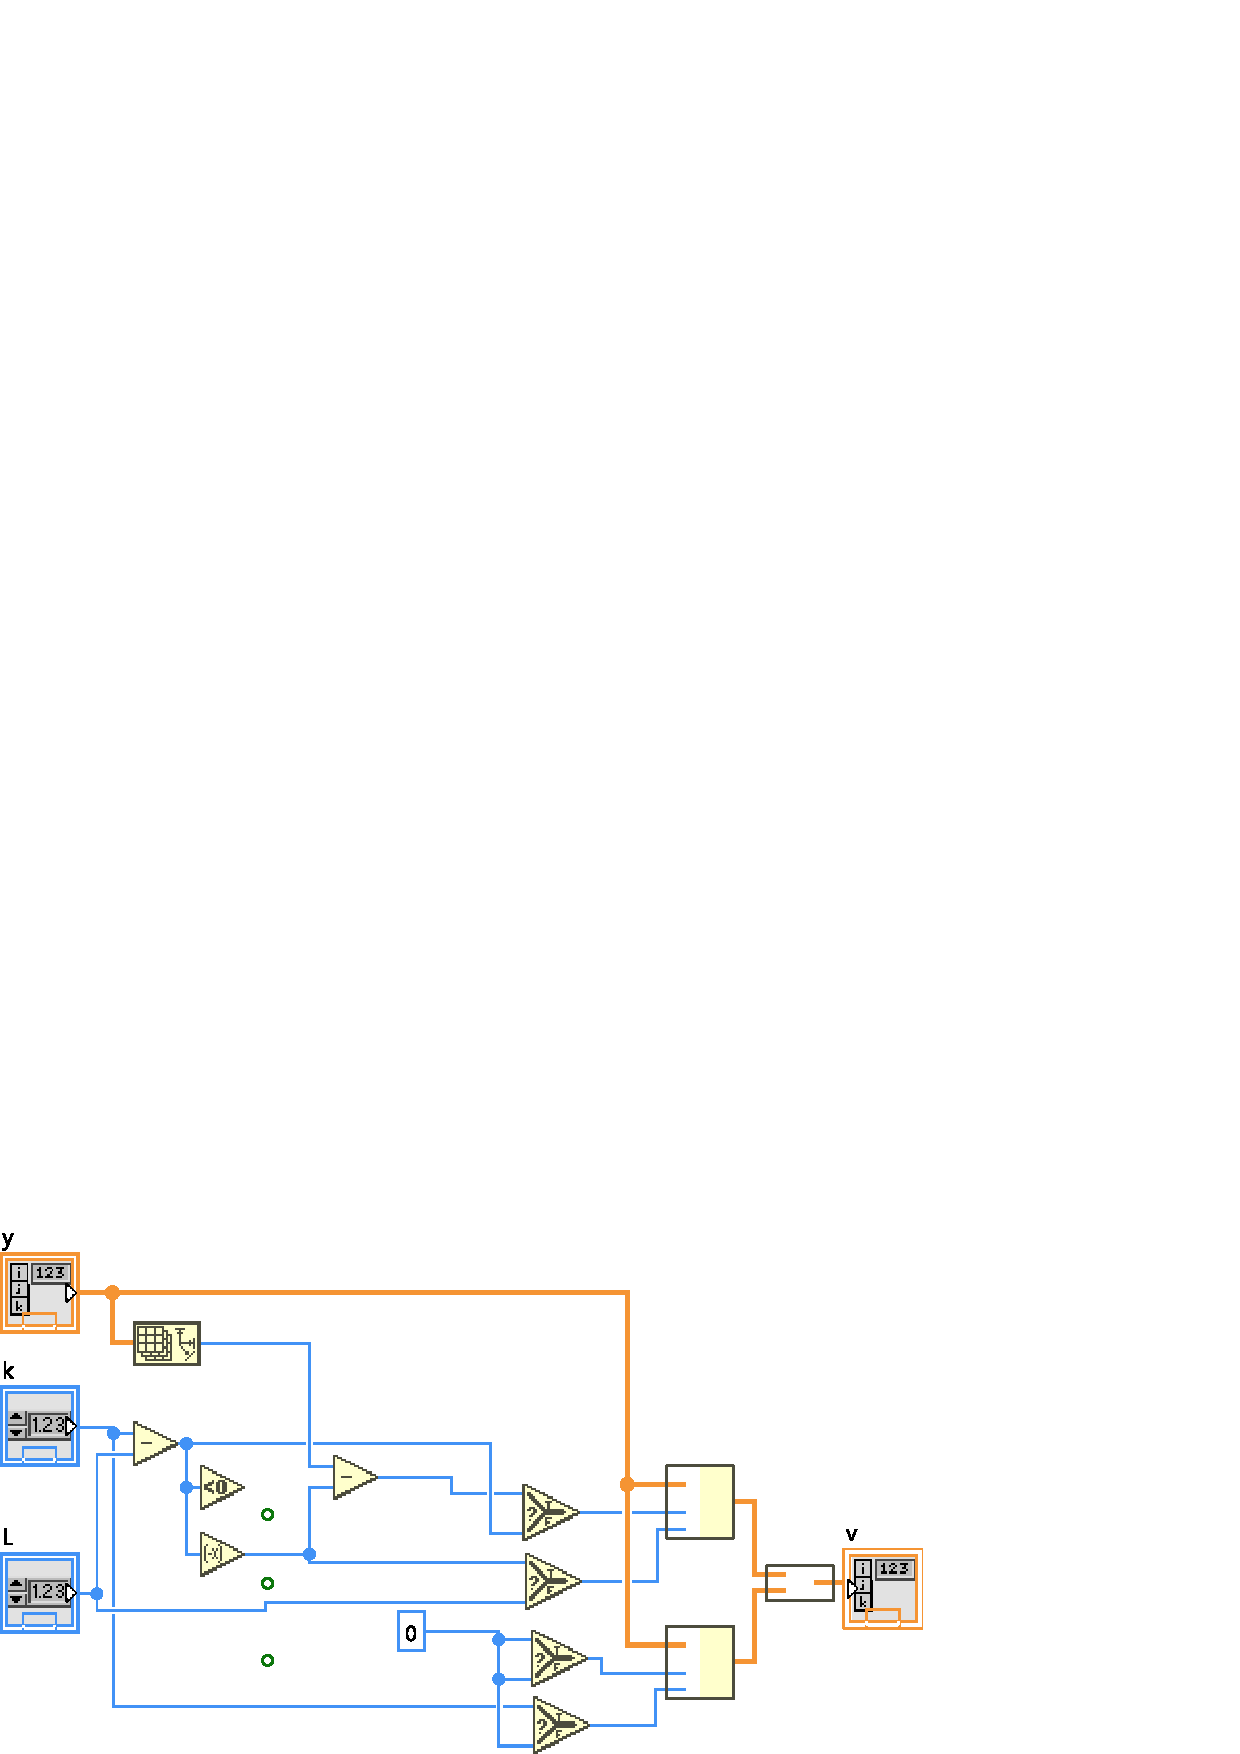
\includegraphics[width=\imsize]{xpstopdf/window.pdf}
    \caption{Diagrama de bloques de la implementación en LabVIEW del módulo que construye una ventana de evaluación $\mathbf{v}$ conteniendo las últimas $L$ muestras registradas en una FIFO cíclica $\mathbf{y}$ a partir del puntero de lectura $k$.\label{fig:window-select-lv}}  
\end{figure}

Las lecturas realizadas sobre $\mathbf{y}$ son por medio de una ventana deslizante, la cual recibe el nombre $\mathbf{v}$. Esta ventana accede a las últimas $N$ muestras registradas en determinado ciclo de iteración, de ser necesario concatenando muestras al final del registro a muestras al inicio del mismo. La asignación de los valores a $\mathbf{v}$ respecto a un puntero de iteración $k$ es la siguiente
\begin{equation}
    \mathbf{v} = \begin{bmatrix}
        y\left[(k-N+1) \bmod L\right], & \cdots, &  y\left[(k-1) \bmod L\right], & y[k]
    \end{bmatrix},
\end{equation}
en donde la longitud de la ventana $L$ es la longitud de la secuencia de entrenamiento de símbolos cortos. En la Figura \ref{fig:window-select-lv} se presenta la esquemática de la implementación en LabVIEW de ésta operación. 

En cada iteración se accede simultáneamente a $\mathbf{y}$ por dos ventanas de evaluación. La primera de estas ventanas es referenciada al instante actual $k$, y se utiliza para calcular los estadísticos $\overline{\Phi}_{BC}$ y $\Phi_{DC}$. La segunda de estas ventanas es referenciada a un ínstante anterior,
\begin{equation}
    k' = (k-2L) \bmod N,
\end{equation}
y se emplea para la estimación del ruido. El desfasaje elegido entre las ventanas es igual al doble de la longitud de la ventana ya que este asegura que ninguna de las muestras utilizadas para estimar el ruido coincida con ninguna de las muestras utilizadas para calcular los estadísticos.


\section{Estrategia de detección}
\label{S:ch5-detección}

El algoritmo de detección consiste en comparar los valores registrados del estadístico de detección con los correspondientes valores registrados del umbral. El registro del estadístico de detección recibirá el nombre de $\upphi$, y este se obtiene de tomar la fila central del registro $\overline{\Phi}_{BC}$. Sin embargo, existen ciertas consideraciones que se deben tomar en un diseño que opera en línea en cuenta para evitar ambugüedad en la detección.

El estadístico de detección produce máximos locales cuando existe presencia parcial de la secuencia de entrenamiento de símbolos cortos en la ventana de evaluación, los cuales pueden superar el umbral de detección. Sin embargo, para realizar el sincronismo temporal, es necesario encontrar el instante óptimo, el cual coincide con la posición del máximo de correlación. En caso de afirmar una detección tan pronto el estadístico exceda el umbral uno corre el riesgo de adelantarse al instante óptimo para el sincronismo. Para evitar este tipo de error, se incluye un tiempo espera, el cual recibe el nombre de $N_{HOLD}$. Éste parámetro representa el número de muestras que esperará el receptor luego de registrar un valor del estadístico que exceda el umbral antes de informar una detección, y será igual a la longitud en muestras de la secuencia de entrenamiento de símbolos cortos.

Por otro lado, es necesario tomar medidas para evitar que una detección sea informada múltiples veces, de lo contrario toda secuencia de entrenamiento de símbolos cortos ya detectada que siga almacenada en $\mathbf{y}$ produciría falsas detecciones en tiempos futuros. Este problema se resuelve considerando dos posibles estados para el receptor: disponible y ocupado. La transición entre el estado ocupado al estado disponible se controla por un parámetro $N_{BUSY}$ que determina el número de muestras que permanecerá el receptor en estado ocupado luego de haber registrado una detección. Este número se elige tal que el receptor regrese al estado disponible cuando la secuencia de entrenamiento de símbolos cortos ya no esté presente en $\mathbf{y}$.

\begin{figure}[t]
    \centering{}\includegraphics[width=\imsizeL]{xpstopdf/detection.pdf}
    \caption{Diagrama de bloques de la implementación en LabVIEW del módulo que implementa el criterio de detección a partir de la comparación del registro del estadístico de detección $\upphi$ contra el registro del umbral $\mathbf{T}$, controlado por los parámetros de epera $T_{HOLD}$ y $T_{BUSY}$.\label{fig:detection-lv}}  
\end{figure}

Tomando en cuenta estas consideraciones, la estrategia para implementar el criterio de detección es la siguiente:
\begin{itemize}
    \item si el receptor está en estado disponible se comparan los registros $\upphi$ y $\mathbf{T}$ elemento a elemento, de modo que cuando suficientes valores registrados en $\upphi$ exceden su correspondiente valor registrado $\mathbf{T}$ se inicializa un contador regresivo con valor $N_{BUSY}$;
    \item en el ciclo de iteración en el cual el contador regresivo alcanza $N_{BUSY}-N_{HOLD}$, se informa la detección por medio de una salida booleana;
    \item en el ciclo de iteración en el cual el contador regresivo alcanza 0, el receptor regresa al estado disponible.
\end{itemize}

En la Figura 5.3 se muestra el esquema de LabVIEW correspondiente a la implementación de la estrategía de detección. Éste módulo cuenta con dos salidas booleanas: \textit{Trigger} estará activa durante un ciclo de iteración para informar que se produjo una detección; y \textit{Busy} permanecerá activa mientras el receptor se encuentre en el estado ocupado.

\section{Estrategia de sincronismo}
\label{S:ch5-sincronismo}

Habiendo tomado las precauciones necesarias para asegurar que no exista más de un preámbulo registrado en $\mathbf{y}$ al momento en el que se informa una detección, se tiene la certeza de que todo inicio de señal entrante está asociada a un valor máximo de los estadísticos de sincronismo dentro de sus respectivos registros de memoria. Por este motivo, no hacen falta más consideraciones que encontrar los valores máximos de cada registro y sus respectivos índices para estimar la muestra inicial y el error de frecuencia correspondiente a cada señal entrante.

\begin{figure}[t]
    \centering{}\includegraphics[width=\imsize]{xpstopdf/bc_sync.pdf}
    \caption{Diagrama de bloques de la implementación en LabVIEW del módulo que implementa el criterio de sincronismo a partir del registro de valores del estadístico proveniente de un banco de correladores contra referencias asociadas a los desvíos en frecuencia de portadora registrados en el parámetro Freqs.\label{fig:bc-sync-lv}}  
\end{figure}

\begin{figure}[t]
    \centering{}\includegraphics[width=\imsize]{xpstopdf/dc_sync.pdf}
    \caption{Diagrama de bloques de la implementación en LabVIEW del módulo que implementa el criterio de sincronismo a partir del registro de valores del estadístico del método $\textit{delay and correlate}$ aplicado a una ventana de $L$ muestras tomadas con un intervalo de muestreo $T_S$.\label{fig:dc-sync-lv}}  
\end{figure}

En la Figura \ref{fig:bc-sync-lv} se presentan las implementaciones en LabVIEW de las estimaciones requeridas para el sistema de sincronismo empleando el banco de correladores, es decir a partir de los valores registrados en $\overline{\Phi}_{BC}$. Asimismo, en la Figura \ref{fig:dc-sync-lv} se muestran las implementaciones de las mismas estimaciones calculadas a través del método delay and correlate, es decir a partir de los valores registrados en $\Phi_{DC}$. Cabe destacar que la estimación de la muestra inicial de recepción es referenciada a la posición de esta muestra en el registro de memoria actual, si se toma en cuenta el índice del ciclo actual se recupera el índice absoluto de la muestra estimada,
\begin{equation}
    \widehat{i} = Nc+\widehat{k}.
\end{equation}

Ambas implementaciones retornan valores contínuamente, pero estos valores solamente se consideran válidos y se registran durante el ciclo de iteración en el que la señal \textit{Trigger} emitida por el módulo de detección toma el valor verdadero.

\section{Visualización de la simulación}

El diagrama de bloques del sistema que se actúa sobre el entorno de simulación presentado en la Figura \ref{fig:top-level-lv} incluye múltiples indicadores, los cuales permiten monitorear el funcionamiento del sistema durante su ejecución, estos son:
\begin{itemize}
    \item FIFO, indicador tipo \textit{waveform graph} que visualiza la parte real e imaginaria del registro $\mathbf{y}$;
    \item Ventana, indicador tipo \textit{waveform graph} que visualiza la ventana sobre la cual se calculan los estadísticos en la iteración actual;
    \item Phi\_DC, indicador tipo \textit{waveform graph} del registro $\Phi_{DC}$, del cual se grafica el módulo y la fase;
    \item Phi\_BC, indicador tipo \textit{intensity graph} del registro $\Phi_{BC}$;
    \item Threshold, indicador tipo \textit{waveform graph} que permite visualizar el umbral junto al estadístico de detección;
    \item Busy, indicador booleano que informa si el receptor se encuentra actualmente en el estado ocupado;
    \item Última Detección, indicador de texto que informa los resultados de las estimaciones de sincronismo pertenecientes a la detección más reciente.
\end{itemize}

\begin{figure}[t]
    \centering{}\includegraphics[width=\imsizeL]{xpstopdf/example_with_sig.pdf}
    \caption{Panel de control de la simulación que evalúa el diseño del sistema de detección y sincronismo implementado, correspondiente al diagrama de bloques presentado en la Figura \ref{fig:top-level-lv}. El panel cuenta con visualizaciones de la señal recibida, los estadísticos de sincronismo, y el estadístico de detección junto con el umbral de decisión. La esquina inferior derecha del panel de control informa las estimaciones de sincronismo correspondientes a la detección más reciente registrada.\label{fig:visualización-lv}}  
\end{figure}

El seguimiento de estos indicadores desde el panel frontal, presentado en la Figura \ref{fig:visualización-lv}, permite verificar que el comportamiento del sistema sea el esperado. Además, el panel frontal provee controladores para la probabilidad de falsa alarma que es utilizada para determinar el umbral de detección, así como para la varianza del ruido y el desvío de frecuencia de portadora que se utilizan para simular las muestras recibidas.


\section{Implementación con procesamiento en \textit{host}}

El diseño desarrollado sobre el entorno de simulación se puede, en principio, traducir de forma directa a un diseño que utiliza un dispositivo NI USRP-2935R para la adquisición de muestras y realiza el procesamiento en el host, esto se consigue remplazando la fuente de datos por la interfaz Rx de la misma. Sin embargo, para la operación en tiempo real la tasa de iteraciones del ciclo de prcesamiento se vuelve un factor limitante, y resulta necesario minimizar el tiempo de ejecución de cada iteración. En primer lugar ésto implica prescindir de las visualizaciones de los registros de memoria, ya que la visualización gráfica es un proceso de alto costo computacional.

\subsection{Limitaciones del diseño}

Al realizar pruebas del sistema con señales adquiridas por el USRP a una tasa de muestreo de 20 MHz se descubrieron las limitaciones del diseño implementado, ya que este no se vio capaz de mantener la tasa de iteraciones requerida para operación en tiempo real. Eventualmente, se provoca error por sobrecarga del \textit{buffer} de recepción en la USRP. Se consideraron dos posibles factores que pueden contribuír a esta sobrecarga: el tiempo de procesamiento requerido por la implementación y el tiempo de lectura requerido para transportar las muestras de la USRP al \textit{host}. 

Considerando que el tiempo de lectura podía ser el factor limitante se propuso reducir el número de lecturas por medio de un diseño alternativo al expuesto anteriormente, el cual permitía leer múltiples muestras presentes en el \textit{buffer} de recepción de la USRP en cada iteración del ciclo principal de procesamiento. Sin embargo, se observó que este diseño alternativo tampoco fue capaz de alcanzar la tasa requerida para mantener la operación en tiempo real, por lo que se decidió no avanzar con el mismo. Los ensayos realizados con el diseño alternativo condujeron a inferir que el factor limitante no es el tiempo de lectura sino el tiempo de procesamiento. 

\color{blue}
\subsection{Análisis de complejidad computacional}

A fin de evaluar la factibilidad de la implementación con procesamiento en \textit{host} se procede a estimar una cota inferior de las operaciones de punto flotante por segundo (FLOPS por su acrónimo en inglés) necesarias para la tasa de iteración requerida, comparada contra una cota superior de las operaciones de punto flotante por segundo que es capaz de alcanzar el CPU del \textit{host}. 

Para estimar la cota inferior de operaciones requeridas por el algoritmo, se parte de cuantificar únicamente la contribución de los productos de correlación, sabiendo que una operación de correlación entre vectores de longitud $L$ se calcula de la siguiente forma
\begin{equation}
    \sum_{n=0}^{L-1}x^\ast[n]y[n],
\end{equation}
en donde los términos son tipo complejo. Una suma de números complejos equivale a 2 operaciones de punto flotante, mientras que un producto de números complejos equivale a 6 operaciones. El producto interno entre vectores de $L$ términos incluye $L$ productos y $L-1$ sumas, las cuales se pueden aproximar a $L$ sumas, teniendo así
\begin{itemize}
    \item $L$ productos complejos $\equiv 6L$ operaciones punto flotante,
    \item $L$ sumas complejas $\equiv 2L$ operaciones punto flotante,
\end{itemize}
lo cual resulta en un total de $8L$ operaciones de punto flotante. El algoritmo diseñado incluye:
\begin{itemize}
    \item $N_F$ productos internos entre vectores de longitud $L$, una por cada referencia en el banco de correladores;
    \item un producto interno entre vectores de longitud $L/2$ para el método \textit{delay and correlate};
    \item un producto interno entre vectores de longitud $L$ para la estimación de la varianza del ruido.
\end{itemize}
En total, las operaciones de producto interno contribuyen $8(N_F+3/2)L$ operaciones de punto flotante por ciclo de iteración. Estas necesitan ser ejecutadas en un tiempo menor o igual a $T_S$ para alcanzar la operación en tiempo real, lo cual resulta en una tasa de operaciones de punto flotante por segundo mínima de
\begin{equation}
    F_{Min} \ge \frac{8(N_F+3/2)L}{T_S}.
\end{equation}
En el caso típico de operación se tienen $L=160$ y $T_S=50$ ns. Si se utilizan 11 referencias para el banco de correladores tal como se hizo en la simulación, se requiere una tasa $F_{Min}\ge 320\text{ GFLOPS}$. 

Por otra parte, una cota superior para la tasa máxima alcanzable por un microprocesador se obtiene de considerar el máximo de su capacidad en condiciones óptimas, dedicando todos sus ciclos de reloj y todos sus núcleos al cálculo numérico y alcanzando a ejecutar el máximo de instrucciones por ciclo de reloj permitidos por la arquitectura, éste valor se obtiene de la siguiente ecuación
\begin{equation}\label{eq:max-flops}
    F_{Max} \le \text{núcleos} \times \frac{\text{ciclos}}{\text{s}}\times\frac{\text{instrucciones}}{\text{ciclo}}.
\end{equation}
El microprocesador con el que cuenta la computadora utilizada es del modelo \textit{Intel Core 2 Quad Q6600}. Este modelo opera a $2.4$ GHz, cuenta con 4 núcleos, e implementa la arquitectura \textit{Intel Core 2} la cual tiene la capacidad de ejecutar 4 operaciones de punto flotante por ciclo de reloj \cite{fog}. Insertando estos valores en la Ecuación \ref{eq:max-flops} se obtiene $F_{Max}\le 38.4$ GFLOPS, el cual es un orden de magnitud menor al mínimo requerido.

\subsection{Evaluación de compromisos para reducir la complejidad computacional}

En vista de los resultados obtenidos del análisis de la complejidad computacional del sistema, se propone y analiza una versión reducida de la implementación. Se considera prescindir del uso del banco de correladores para el sincronismo y usar únicamente el método \textit{delay and correlate} para este propósito, mientras que la correlación con la secuencia de entrenamiento de símbolos cortos en ausencia de error de frecuencia se calcula para propósitos de detección. Se propone, además, utilizar una menor cantidad de muestras para la estimación de la varianza del ruido, nominalmente reducir el número de muestras utilizadas a la mitad. 

Aplicando estas limitaciones al sistema, se reduce la contribución de los productos internos a únicamente $16L$ operaciones de punto flotante por ciclo de iteración. En la operación típica esto corresponde a un requerimento de $F_{Min} \ge 51.2$ GFLOPS. Sin embargo, este valor sigue excediendo el máximo teórico del microprocesador, volviendo inviable proceder con este método.


\color{black}

\section{Conclusiones del capítulo}

Se consiguió implementar un diseño que integre los algoritmos de detección y sincronismo detallados en los capítulos anteriores, el cual aplica estrategias para resolver el problema de las ambigüedades en la detección propias a la operación en tiempo real. El funcionamiento diseño implementado pudo ser verificado exitosamente dentro de un entorno de simulación a modo de prueba de concepto.

Sin embargo, al momento de implementar el diseño utilizando las muestras adquiridas por una USRP como fuente de datos, se encontró que este no es capaz de alcanzar la tasa de iteraciones requerida para el funcionamiento en tiempo real, y se concluyó que el tiempo de procesamiento en CPU es el factor limitante. Del estudio realizado sobre el hardware disponible y las herramientas de desarrollo asociadas surgen dos alternativas para resolver el cuello de botella que produce el tiempo del procesamiento. Una alternativa es avanzar con optimizaciones sobre el diseño, realizando un análisis de la complejidad algorítmica del mismo y buscando estrategias para reducir el número de operaciones de punto flotante realizadas en cada iteración. Otra posibilidad implica estudiar en mayor profundidad los métodos para desarrollar módulos personalizados con LabVIEW-FPGA y transportar las etapas del procesamiento computacionalmente costosas a la FPGA interna de la USRP. 

Si bien ambos caminos para avanzar hacia el objetivo de operación en tiempo real cuentan con su grado de complejidad, cabe mencionar que no son mutuamente excluyentes, ya que las optimizaciones algorítmicas que se realicen sobre el diseño que se ejecuta en el \textit{host} también podrán aplicarse a la versión del diseño que se sintetizaría en la FPGA. 





%%% Local Variables: 
%%% mode: latex
%%% TeX-master: "template"
%%% End: 

\chapter{Conclusiones}
\label{Ch:6}
\graphicspath{{figs/}}
%%%%%%%%%%%%%%%%%%%%%%%%%%%%%%%%%%%%%%%%%%%%%%%%%%%%%%%%%%%%%%%%%%%%%%%%

A lo largo de este trabajo se logró implementar en LabVIEW los algoritmos de detección y sincronismo para señales que emplean OFDM de acuerdo al estándar IEEE 802.11, y se consiguió integrar a estos en un sistema que es capaz de ejecución continua sobre una secuencia de muestras en banda base provenientes de la recepción. Durante el diseño de este sistema se identificaron posibles fuentes de error en los resultados de los algoritmos propias del funcionamiento en tiempo real, y se definieron e implementaron medidas para evitar tales errores. 

El funcionamiento del sistema implementado se verificó por medio de un entorno de simulación que aproxima al problema real, validando que no se produzcan detecciones erroneas evitables y que los algoritmos de sincronismo se apliquen en un momento adecuado y retornen los resultados esperados. La ejecución del sistema implementado sobre el entorno de simulación resultó en una exitosa prueba de concepto a nivel lógico del sistema.

En la etapa siguiente del desarrollo se buscó la implementación del sistema sobre señales reales, utilizando un dispositivo NI USRP-2953R para la adquisición de las muestras y realizando el procesamiento de las mismas dentro de la computadora. En esta etapa se identificaron las limitaciones del sistema al este ser ejecutado en la computadora, ya que en estas condiciones no es capaz de alcanzar la mínima tasa de iteraciones requerida para mantener la recepción en tiempo real de señales transmitidas de acuerdo al estándar IEEE 802.11. Fue posible determinar que el factor limitante es el tiempo de procesamiento en la computadora, y no el tiempo de comunicación por puerto serie entre la computadora y la USRP.

Estos pasos se consideran necesarios para el eventual desarrollo de un sistema que cumpla los requisitos, ya que se identificó que el siguiente paso recomendado es la implementación de los algoritmos computacionalmente costosos en la FPGA interna del dispositivo USRP. En la última etapa del trabajo se llegó a analizar la posibilidad de la implementación en FPGA del sistema, pero esta demostró no ser problema menor, ya que requiere tanto de la descripción y síntesis de módulos LabVIEW FPGA personalizados como de modificaciones de la interfaz de \textit{device} a \textit{host} de la USRP para permitir acceso a los resultados de los algoritmos.

\section{Trabajo futuro}
\label{S:trabajo-futuro}

En base a los resultados de este proyecto, una vía natural de trabajo a futuro es el estudio más extenso de las herramientas LabVIEW FPGA, ya que se considera que la implementación de los algoritmos en FPGA representa el siguiente paso requerido para alcanzar los objetivos de operación en tiempo real del sistema de detección y sincronismo que fue desarrollado.

Otra vía de trabajo a futuro posible consiste en avanzar en las etapas de procesamiento requeridas para la recepción de señales genradas de acuerdo al estándar IEEE 802.11. Esta vía continuaría con un estudio en mayor profundidad de la secuencia de entrenamiento de símbolos largos, la cual no fue utilizada en los algoritmos implementados en este proyecto. En base a esa secuencia de entrenamiento se puede proceder a implementar algoritmos para la estimación del canal inalámbrico, y eventualmente incorporar los resultados de sincronismo y estimación del canal para la demodulación del símbolo SIGNAL. 


%\appendix
%\include{apend1}

\begin{biblio}
\bibliography{mibib}
\end{biblio}


\begin{postliminary}

%\begin{seccion}{Publicaciones asociadas}
%  \begin{enumerate}
%  \item Mi primer aviso en la revista \textbf{ABC}, 1996
%  \item Mi segunda publicaci\'{o}n en la revista \textbf{ABC}, 1997
%  \end{enumerate}
%\end{seccion}

\begin{seccion}{Agradecimientos}
A todos los que se lo merecen, por merecerlo
\end{seccion}

\end{postliminary}

\end{document}

 